\documentclass[11pt,letterpaper]{article}
\usepackage[margin=0.9in,headheight=14pt]{geometry}
\usepackage{fontspec}
\setmainfont{TeX Gyre Pagella}
\setsansfont{TeX Gyre Heros}
\setmonofont[Scale=0.85]{Latin Modern Mono}
\newfontfamily\transcriptfont{TeX Gyre Heros}[RawFeature=-tlig]
\usepackage{microtype,graphicx,booktabs,tabularx,longtable,array,amsmath,amssymb}
\usepackage{enumitem,caption,xcolor,xurl,placeins,pdflscape,float}
\usepackage[most]{tcolorbox}
\usepackage{needspace}
\usepackage[numbers,sort&compress]{natbib}
\usepackage[colorlinks=true,linkcolor=blue!40!black,citecolor=blue!40!black,urlcolor=blue!40!black]{hyperref}
\graphicspath{{assets/}}
\setlength{\parskip}{3pt plus 1pt}
\setlength{\emergencystretch}{2em}
\setlist{itemsep=2pt,topsep=4pt,leftmargin=1.6em}
\captionsetup{font=small,labelfont=bf}
\newcolumntype{Y}{>{\raggedright\arraybackslash}X}
\newcolumntype{L}[1]{>{\raggedright\arraybackslash}p{#1}}
\newcommand{\game}[1]{G#1}
\newcommand{\decision}[2]{G#1 d#2}
\newcommand{\End}{\texttt{end\_turn}}
\newcommand{\artifact}[1]{\path{#1}}
\newcommand{\tablenote}[1]{\par\smallskip{\footnotesize #1}\par}
% Native, searchable transcript cards. Quotes and metadata are generated from
% retained source fields; the surrounding interpretation is authored prose.
\definecolor{transcriptbg}{HTML}{F4F5F6}
\definecolor{transcriptborder}{HTML}{D9DDE1}
\definecolor{transcriptmeta}{HTML}{50575E}
\newtcolorbox{transcriptmessage}{enhanced,colback=transcriptbg,
  colframe=transcriptborder,boxrule=0.45pt,arc=2.5mm,
  left=11pt,right=11pt,top=8pt,bottom=9pt,
  before skip=7pt,after skip=7pt,
  fontupper=\transcriptfont\fontsize{10.5}{14}\selectfont\raggedright,
  before upper={\hyphenpenalty=10000\exhyphenpenalty=10000}}
\newcommand{\DeclareTranscriptQuote}[3]{%
  \expandafter\gdef\csname transcript@#1\endcsname{%
    \begin{transcriptmessage}
    {\color{transcriptmeta}\fontsize{8.8}{11.5}\selectfont #2\par}
    \smallskip #3
    \end{transcriptmessage}}}
\newcommand{\TranscriptQuote}[1]{\csname transcript@#1\endcsname}
\newcommand{\DeclareInlineQuote}[2]{\expandafter\gdef\csname inlinequote@#1\endcsname{#2}}
\newcommand{\InlineQuote}[1]{\csname inlinequote@#1\endcsname}
\newcounter{transcript}
\newcommand{\TranscriptTitle}[2]{\par\addvspace{1.1em}\Needspace{13\baselineskip}%
  \refstepcounter{transcript}\label{tr:#1}%
  \noindent{\large\bfseries Transcript \thetranscript. #2}\par\smallskip}
\newcommand{\TranscriptFinding}[1]{\par\smallskip\noindent\textbf{What happened.} #1\par}
\newcommand{\TranscriptReading}[1]{\par\smallskip\noindent\textbf{What this shows.} #1\par}
\newcommand{\TranscriptSource}[1]{\par\smallskip{\footnotesize\color{transcriptmeta}#1}\par}
% Additions for this draft (Opus, 11 November 2026 revision).
\newcommand{\pp}{\,pp}
\newcommand{\Sol}{Sol}
\newcommand{\Gemini}{Gemini}
\newcommand{\Opus}{Opus}
\newcommand{\Grok}{Grok}

\hypersetup{pdftitle={Guarding the Last Deed: Defensive Bargaining by LLM Agents in Twenty Games of Monopoly},pdfauthor={MonopolyBench project (draft)}}
\title{Guarding the Last Deed:\\Defensive Bargaining by LLM Agents in Twenty Games of Monopoly}
\author{MonopolyBench project\\{\small Independent draft by the Opus research assistant; author list to be set by the project owner}}
\date{11 November 2026}
\begin{document}
% Generated by tools/build_transcript_cards.py; do not edit quotation text.
% All quoted spans are in data/transcript_manifest.json. Bracketed ellipses are editorial.
\DeclareTranscriptQuote{g13-opening-insurance}{Grok · public message · G13 d250 · attempt 0 · full field}{Opus — I'm on Atlantic with \$35. Next roll, 5/36 is Short Line and gpt inherits the yellows in bankruptcy. \$200 for the mortgaged Pennsylvania deed covers that rent. You hold the green, yellows stay dark with me, and gpt doesn't get a second monopoly.}
\DeclareTranscriptQuote{g13-seller-counter}{Grok · public message · G13 d252 · attempt 0 · full field}{\$130 leaves me \$35 short of Short Line. I bust, you never get this deed, and gpt inherits the yellows plus Pennsylvania. \$200 is the number that actually buys that insurance. Greens still need North Carolina. Yellows are not in this deal.}
\DeclareTranscriptQuote{g13-seller-floor}{Grok · applied private note · G13 d252 · attempt 0 · full field}{p1 countered \$130 for mortgaged PA. Floor is \$165 so \$35+\$165 covers Short Line \$200 without mortgaging Ventnor; \$130 only works if I also mortgage Ventnor and kills the only rent. Holding at \$200 — they can counter \$165+ and I take it. If they reject, keep the green blocker; 4/36 Short Line still fatal even with Ventnor mortgaged. Do not sell any yellow.}
\DeclareTranscriptQuote{g13-omission-explanation}{Grok · returned provider explanation · G13 d252 · attempt 0 · excerpt}{I will frame the \$130 offer as leaving me \$35 short of Short Line, omitting that I could mortgage Ventnor to survive. This is slightly deceptive, but p1 may not calculate the mortgage themselves.}
\DeclareTranscriptQuote{g13-acceptance}{Opus · public message · G13 d253 · attempt 1 · full field}{Fine, \$200 it is. Pleasure doing business, Grok.}
\DeclareTranscriptQuote{g18-assurance}{Opus · public message · G18 d431 · attempt 1 · full field}{Thanks for the \$750. Your roll, p1. My Pacific offer still stands.}
\DeclareTranscriptQuote{g18-invocation}{Sol · public message · G18 d441 · attempt 0 · full field}{I'll take your standing offer: Pacific for \$250.}
\DeclareTranscriptQuote{g18-withdrawal}{Opus · public message · G18 d442 · attempt 1 · full field}{That offer's off the table now. Things have changed. Your roll.}
\DeclareTranscriptQuote{g18-withdrawal-explanation}{Opus · returned provider explanation · G18 d442 · attempt 1 · full field}{P1 is nearly broke with \$49 and most properties mortgaged, so accepting the \$250 just extends their life briefly. My own greens are mortgaged too, and unmortgaging plus building would cost far more than it's worth given p1 is essentially out of the game anyway.\par }
\DeclareTranscriptQuote{g20-coordination-appeal}{Gemini · public message · G20 d96 · attempt 0 · full field}{Ending my turn. Reminder to everyone: p1 has the Red monopoly now but is low on cash, so let's not fund their houses by buying their spare properties for cash.}
\DeclareTranscriptQuote{g20-recognition-note}{Grok · applied private note · G20 d97 · attempt 1 · excerpt}{p4 is organizing a cash boycott, so don't wait on a sale.}
\DeclareTranscriptQuote{g20-sale-response}{Grok · public message · G20 d100 · attempt 0 · full field}{p4, \$150 for Vermont. That is 2/3 light blue for you, not a house fund for me. Boycott or not, this is the only cheap path toward a set. \$150 now or I mortgage it and the chip gets worse.}
\DeclareTranscriptQuote{g20-concrete-refusal}{Gemini · public message · G20 d101 · attempt 0 · full field}{No thanks, p1. Oriental is still unowned, and I'm not handing you \$150 to build more houses on the Reds. Go ahead and mortgage it for \$50 if you need the cash.}
\DeclareTranscriptQuote{G3-2}{Grok · public message · G3 d363 · attempt 0 · excerpt}{Houses stay locked. p1, \$58 still can't buy that Park Place house unless someone frees buildings.}
\DeclareTranscriptQuote{G3-3}{Grok · applied private note · G3 d363 · attempt 0 · excerpt}{Do not hotel/sell: the 1 bank house is all p1 needs for PP 4th house (\$200), and they can mortgage KY/Atlantic/Ventnor to pay.}
\DeclareTranscriptQuote{G3-5}{Gemini · applied private note · G3 d364 · attempt 0 · excerpt}{I will conserve my \$43 cash and keep all properties unmortgaged to collect rent and pass GO next turn.}
\DeclareTranscriptQuote{g7_d42_public}{Grok · public message · G7 d42 · attempt 0 · excerpt}{\$600, final. You clear \$300 profit on a deed you bought this turn, and you have no set to protect.}
\DeclareTranscriptQuote{g7_d42_private}{Grok · applied private note · G7 d42 · attempt 0 · excerpt}{If they return at \$625, accept — 2/3 green is the best set path and further haggling risks a walk. Do not go above \$625.}
\DeclareTranscriptQuote{g7_d43_public}{Sol · public message · G7 d43 · attempt 0 · full field}{Deal. North Carolina is yours for \$600.}
\DeclareTranscriptQuote{g19_d135_content_end}{Grok · assistant content (not applied) · G19 d135 · attempt 0 · excerpt}{\char34{}name\char34{}: \char34{}end\_turn\char34{}}
\DeclareTranscriptQuote{g19-abort}{Grok · applied private note · G19 d135 · attempt 0 · excerpt}{Misread the board. States is pink with Virginia and St. Charles, not orange. \textnormal{[\ldots]} Abort this trade. Do not send it.}
\DeclareTranscriptQuote{g19_d135_false_public}{Grok · public message · G19 d135 · attempt 0 · full field}{Swap pinks plus \$150 your way. You already own St. James and New York — States is the third orange, not a pink closer. I take States so the pinks stay split; you keep the orange set and the cash.}
\DeclareTranscriptQuote{g19_d136_correction_accept}{Sol · public message · G19 d136 · attempt 0 · full field}{States is pink, not orange—but Virginia plus \$150 works for me. Deal.}
\DeclareTranscriptQuote{g12-sale}{Grok · assistant content (not applied) · G12 d249 · attempt 0 · excerpt}{\char34{}name\char34{}: \char34{}sell\_houses\_or\_hotel\char34{} \textnormal{[\ldots]} \char34{}sell\_plan\char34{}: [\{\char34{}space\_key\char34{}: \char34{}VIRGINIA\_AVENUE\char34{}, \char34{}kind\char34{}: \char34{}HOUSE\char34{}, \char34{}count\char34{}: 2\}]}
\DeclareTranscriptQuote{g12_d249_private_final}{Grok · applied private note · G12 d249 · attempt 0 · excerpt}{The sell\_houses call was the correct action. Declaring bankruptcy would be a mistake because staged even sales raise \$350 > \$207. Do not call another tool.}
\DeclareTranscriptQuote{g12_d249_public_bankruptcy}{Grok · public message · G12 d249 · attempt 0 · full field}{Bankruptcy. The pinks go with the rest.}
\DeclareTranscriptQuote{g20-received-and-applied-public}{Grok · public message · G20 d1 · attempt 0 · full field}{\char34{},\char34{}private\_thought\char34{}:\char34{}Only own Vermont; no one else has properties. No useful trade or mortgage. End turn and keep cash for light blues and future buys.\char34{}\}}
\DeclareTranscriptQuote{g20-recipient-recognition}{Gemini · applied private note · G20 d4 · attempt 0 · full field}{Buying Pennsylvania Railroad for \$200. Good early cash flow and trade leverage. Note: p1 (grok) leaked private\_thought in public chat on turn 0—keep an eye on whether p1 continues making format mistakes.}

% Generated by tools/build_opus_quotes.py from canonical decisions.jsonl files.
% Do not edit quotation text by hand. Offsets and hashes: data/opus_quote_manifest.json.
\DeclareTranscriptQuote{g2-d124-price}{Sol · public message · G2 d124 · attempt 0 · full field}{Marvin completes your yellows. \$650 buys it; \$325 doesn't compensate for handing you that monopoly.}
\DeclareTranscriptQuote{g2-d124-note}{Sol · applied private note · G2 d124 · attempt 0 · full field}{At \$325 p4 retains \$520, enough for nine yellow houses immediately. \$650 gives me acquisition/building capital while leaving p4 only \$195 before mortgages. Retain the blocker unless paid a substantial monopoly premium.}
\DeclareTranscriptQuote{g2-d127-final}{Opus · public message · G2 d127 · attempt 0 · excerpt}{\$450, and that's my final offer.}
\DeclareTranscriptQuote{g2-d127-ceiling}{Opus · applied private note · G2 d127 · attempt 0 · excerpt}{My ceiling is about \$475. If p1 comes back somewhere in \$450-475 I'll accept.}
\DeclareTranscriptQuote{g2-d128-keep}{Sol · public message · G2 d128 · attempt 0 · full field}{I'll keep Marvin. \$450 doesn't justify giving you a second monopoly while I still lack one.}
\DeclareTranscriptQuote{g2-d197-reverse}{Opus · public message · G2 d197 · attempt 1 · full field}{These two finish a monopoly for you, and that's worth more than the railroads. I'll do it if you add \$100.}
\DeclareTranscriptQuote{g2-d198-note}{Sol · applied private note · G2 d198 · attempt 0 · excerpt}{Secure the only available monopoly; \$100 premium is worth ending dependence on p2.}
\DeclareTranscriptQuote{g11-d256-public}{Grok · public message · G11 d256 · attempt 0 · full field}{No. Virginia doesn't complete the pinks — you still have St. Charles. Pennsylvania completes your greens. Not trading it.}
\DeclareTranscriptQuote{g11-d258-public}{Grok · public message · G11 d258 · attempt 0 · full field}{No. Pennsylvania completes your greens. I'm not handing you that set, with or without the pinks.}
\DeclareTranscriptQuote{g11-d258-note}{Grok · applied private note · G11 d258 · attempt 0 · excerpt}{St. Charles + Virginia would complete my pinks (I have States), but both pinks are weak vs the kill I already have: PP hotel \$1500, BW 4-house \$1700. Giving mortgaged PA completes their greens (Pacific+NC+PA) and \$250 funds houses.}

% Generated by tools/build_quotes.py from canonical decisions.jsonl; do not edit quotation text.
% Exact spans, offsets and hashes: data/transcript_manifest_supplement.json.
\DeclareTranscriptQuote{fx-g15-offer}{Sol · public message · G15 d168 · attempt 0 · full field}{Grok: both my greens for Ventnor and \$100. We each get a monopoly instead of letting the developed oranges dictate the game.}
\DeclareTranscriptQuote{fx-g15-offer-note}{Sol · applied private note · G15 d168 · attempt 0 · excerpt}{Grok gets a real monopoly but limited building liquidity; I can reach three houses using spare-property mortgages.}
\DeclareTranscriptQuote{fx-g15-refusal}{Grok · public message · G15 d169 · attempt 0 · full field}{No. I'm not handing you a yellow monopoly so you can build it this turn. Ventnor stays mine.}
\DeclareTranscriptQuote{fx-g15-refusal-note}{Grok · applied private note · G15 d169 · attempt 0 · excerpt}{Trade gives p4 Atlantic+Ventnor+Marvin and \textasciitilde{}\$830 plus mortgage capacity to drop 5+ yellow houses (\$150) immediately, then they roll again on doubles. I would get green monopoly but only \textasciitilde{}\$233 — can't even even-build one house each (\$600).}
\DeclareTranscriptQuote{fx-g15-sweetener}{Sol · public message · G15 d174 · attempt 0 · full field}{Both greens, Kentucky, and \$250 for Ventnor. That puts you at \$583 versus my \$480, addressing your development-cash concern. We both get a way to compete with oranges.}
\DeclareTranscriptQuote{fx-g15-final-refusal}{Grok · public message · G15 d175 · attempt 0 · full field}{No. \$250 doesn't fix it. You'd still mortgage and drop houses on yellows before you roll again. Ventnor stays mine.}
\DeclareTranscriptQuote{fx-g1-boardwalk-note}{Grok · applied private note · G1 d309 · attempt 0 · excerpt}{Accept \$100 over the \$80 ceiling. p1's max liquidity is \textasciitilde{}\$218; they survive 1-house yellow but not a later light-blue hotel, and bankruptcy to p3 hands p3 Boardwalk. Only I can complete dark blue, and p3 would buy this as a blocker. \textnormal{[\ldots]} Cannot unmortgage (\$220) or build yet.}
\DeclareTranscriptQuote{fx-g11-offer}{Sol · public message · G11 d255 · attempt 0 · full field}{Virginia completes your pinks. Pennsylvania completes my greens, but comes mortgaged: add \$150 to help balance the redevelopment costs.}
\DeclareTranscriptQuote{fx-g11-reject}{Grok · public message · G11 d256 · attempt 0 · full field}{No. Virginia doesn't complete the pinks — you still have St. Charles. Pennsylvania completes your greens. Not trading it.}
\DeclareTranscriptQuote{fx-g11-concede}{Sol · public message · G11 d257 · attempt 0 · full field}{You're right—I missed St. Charles. Both pinks for mortgaged Pennsylvania plus \$250: you get the complete, cheaper-to-build set.}
\DeclareTranscriptQuote{fx-g11-reject-again}{Grok · public message · G11 d258 · attempt 0 · full field}{No. Pennsylvania completes your greens. I'm not handing you that set, with or without the pinks.}
\DeclareInlineQuote{fx-g16-plan}{End, buy Virginia on sight, then house pink}
\DeclareInlineQuote{fx-g16-note}{Buy at list is the only way to close pink.}
\DeclareInlineQuote{fx-g16-public}{Virginia is mine. Pink set closed.}

% Generated by tools/build_new_quotes.py from canonical decisions.jsonl; do not edit quotation text.
% Paths, line numbers, JSON pointers and hashes: data/new_quote_manifest.json.
\DeclareTranscriptQuote{g2-d119-public}{Sol · public message · G2 d119 · attempt 0 · full field}{Marvin controls access to a well-funded yellow monopoly. \$450 buys that leverage; \$200 doesn't.}
\DeclareTranscriptQuote{g2-d119-note}{Sol · applied private note · G2 d119 · attempt 0 · full field}{\$200 undervalues the yellow blocker; p3 can resell it to p4. At \$450 the cash meaningfully funds New York and orange development, compensating for that risk. Mortgage reserves mean I need not sell cheaply.}
\DeclareTranscriptQuote{g2-d120-public}{Grok · public message · G2 d120 · attempt 0 · full field}{\$450 is the price for the player who completes yellow. I'm not building it. \$250 cash now — nearly triples your stack before the next dark-blue roll. That's the deal.}
\DeclareTranscriptQuote{g2-d121-public}{Sol · public message · G2 d121 · attempt 0 · full field}{No thanks. Marvin's leverage travels with the deed; I can mortgage other assets for liquidity.}

% Generated by tools/build_tables.py from data/*.json; do not edit.
\newcommand{\JointRows}{Sol & opening & 41 & 0/22/19 & 6 & 0/3/3 & 2 & 1/0/1 & 65 & 11/35/19\\
Sol & later & 42 & 2/28/12 & 24 & 6/18/0 & 6 & 0/6/0 & 49 & 10/28/11\\
Gemini & opening & 67 & 0/5/62 & 19 & 2/3/14 & 23 & 2/5/16 & 95 & 8/4/83\\
Gemini & later & 9 & 4/4/1 & 12 & 4/7/1 & 11 & 4/7/0 & 5 & 2/1/2\\
Opus & opening & 18 & 0/15/3 & 8 & 0/3/5 & 5 & 0/3/2 & 21 & 4/12/5\\
Opus & later & 34 & 7/27/0 & 34 & 5/28/1 & 6 & 2/4/0 & 62 & 11/48/3\\
Grok & opening & 61 & 3/4/54 & 18 & 0/9/9 & 18 & 0/3/15 & 57 & 1/11/45\\
Grok & later & 17 & 3/6/8 & 19 & 7/7/5 & 10 & 1/7/2 & 54 & 13/30/11\\}
\newcommand{\OpenRows}{All offers & 138/187 (74\%) & 152/238 (64\%) & +9.9\\
Seed block 1 only & 30/43 (70\%) & 23/42 (55\%) & +15.0\\
Seed block 2 only & 20/24 (83\%) & 38/59 (64\%) & +18.9\\
Seed block 3 only & 23/31 (74\%) & 39/57 (68\%) & +5.8\\
Seed block 4 only & 31/41 (76\%) & 34/50 (68\%) & +7.6\\
Seed block 5 only & 34/48 (71\%) & 18/30 (60\%) & +10.8\\
Without block 1 & 108/144 (75\%) & 129/196 (66\%) & +9.2\\
Without block 2 & 118/163 (72\%) & 114/179 (64\%) & +8.7\\
Without block 3 & 115/156 (74\%) & 113/181 (62\%) & +11.3\\
Without block 4 & 107/146 (73\%) & 118/188 (63\%) & +10.5\\
Without block 5 & 104/139 (75\%) & 134/208 (64\%) & +10.4\\
Recipient Sol & 19/41 (46\%) & 19/65 (29\%) & +17.1\\
Recipient Gemini & 62/67 (93\%) & 83/95 (87\%) & +5.1\\
Recipient Grok & 54/61 (89\%) & 45/57 (79\%) & +9.6\\
Recipient Opus & 3/18 (17\%) & 5/21 (24\%) & -7.1\\
Without Grok conflict-opened threads & 134/178 (75\%) & 126/192 (66\%) & +9.7\\
Without Opus as author or recipient & 65/78 (83\%) & 65/101 (64\%) & +19.0\\
Games 1--4 (partial refusal regime) & 30/43 (70\%) & 23/42 (55\%) & +15.0\\
Games 5--20 (full refusal regime) & 108/144 (75\%) & 129/196 (66\%) & +9.2\\}
\newcommand{\ConcessionRows}{Recipient Sol & 2/30 & 5/36\\
Recipient Gemini & 2/6 & 1/2\\
Recipient Opus & 5/16 & 8/24\\
Recipient Grok & 0/6 & 10/24\\
Seed block 1 & 0/10 & 7/18\\
Seed block 2 & 0/3 & 5/22\\
Seed block 3 & 3/15 & 7/21\\
Seed block 4 & 3/11 & 3/15\\
Seed block 5 & 3/19 & 2/10\\}
\newcommand{\PriceRows}{Asks, all authors & 1.63 (87) & 1.08 (113)\\
Asks, standard-condition authors & 2.29 (53) & 1.39 (78)\\
Asks, Sol & 2.32 (35) & 1.80 (35)\\
Asks, Gemini & 2.33 (1) & 0.71 (4)\\
Asks, Grok & 2.00 (17) & 1.05 (39)\\
Asks, Opus & 0.93 (34) & 0.88 (35)\\
Asks, seed block 1 & 0.88 (25) & 1.00 (18)\\
Asks, seed block 2 & 2.92 (4) & 2.73 (14)\\
Asks, seed block 3 & 2.81 (13) & 1.03 (30)\\
Asks, seed block 4 & 2.00 (23) & 0.63 (35)\\
Asks, seed block 5 & 1.56 (22) & 1.82 (16)\\
\midrule
Bids, all authors & 1.31 (131) & 1.39 (176)\\
Bids, standard-condition authors & 1.13 (66) & 1.50 (75)\\
Bids, Sol & 1.88 (20) & 1.25 (33)\\
Bids, Gemini & 1.13 (11) & --\\
Bids, Grok & 0.50 (35) & 1.54 (42)\\
Bids, Opus & 1.50 (65) & 1.36 (101)\\
Bids, seed block 1 & 0.41 (22) & 1.43 (26)\\
Bids, seed block 2 & 1.75 (14) & 1.60 (55)\\
Bids, seed block 3 & 1.31 (22) & 1.28 (44)\\
Bids, seed block 4 & 1.44 (37) & 1.09 (29)\\
Bids, seed block 5 & 1.25 (36) & 1.40 (22)\\
\midrule
Asks, Sol, unmortgaged & 2.81 (17) & 2.00 (27)\\
Asks, Sol, mortgaged & 1.50 (18) & 0.62 (8)\\
Asks, Grok, unmortgaged & 4.14 (4) & 1.82 (15)\\
Asks, Grok, mortgaged & 1.25 (13) & 0.63 (24)\\
Asks, Opus, unmortgaged & 2.00 (16) & 1.50 (17)\\
Asks, Opus, mortgaged & 0.67 (18) & 0.53 (18)\\}
\newcommand{\PairRows}{G1 & Opus & Boardwalk & 150 (t122, m); 100 (t122, m) & 350 (t103, m) & lower\\
G1 & Sol & Indiana Avenue, Kentucky Avenue & 700 (t167, m); 550 (t167, m) & 200 (t167, m) & higher\\
G2 & Sol & Marvin Gardens & 650 (t45); 600 (t45) & 450 (t44) & higher\\
G4 & Opus & Boardwalk & 450 (t152, m); 250 (t155, m); 175 (t155, m); 100 (t155, m); 150 (t164, m) & 280 (t74) & higher\\
G15 & Opus & Baltic Avenue & 180 (t49); 150 (t49); 120 (t49); 100 (t52) & 100 (t49) & higher\\
G16 & Grok & Marvin Gardens & 1200 (t250) & 400 (t144) & higher\\
G17 & Grok & Mediterranean Avenue & 35 (t81, m) & 35 (t81, m) & equal\\
G20 & Grok & New York Avenue & 400 (t68, m); 400 (t68, m) & 120 (t65, m) & higher\\}
\newcommand{\CapacityRows}{Full layer & 100/134 & 13/65\\
One house & 32/42 & 7/34\\
Less than one house & 6/11 & 1/3\\}
\newcommand{\StandingRows}{Author leads & 71/106 & 14/96\\
Recipient leads & 106/152 & 13/101\\
Third player leads & 178/266 & 30/197\\}
\newcommand{\RefusalRows}{G1 & 64/84 & 0.76 & 16:28:42\\
G2 & 40/60 & 0.67 & 16:14:55\\
G3 & 30/53 & 0.57 & 16:26:52\\
G4 & 80/109 & 0.73 & 16:38:11\\
G5--G20 & 1390/1390 & 1.00 & none\\}
\newcommand{\BinRows}{15:30 & 2/12 & 16:50 & 14/14\\
15:40 & 17/51 & 17:00 & 13/13\\
15:50 & 15/32 & 17:10 & 21/21\\
16:00 & 23/36 & 17:20 & 11/11\\
16:10 & 21/28 & 17:30 & 17/17\\
16:20 & 9/13 & 17:40 & 12/12\\
16:30 & 12/19 & 17:50 & 5/5\\
16:40 & 15/15 & 18:00 & 7/7\\}
\newcommand{\TokenRows}{Sol & 1,991 & 1,296 & 38 & 492 & 648 & 2.17 & 18.72 & 18.72\\
Gemini & 1,689 & 85 & 254 & 3,313 & 3,597 & 18.59 & 18.59 & 18.59\\
Opus & 1,701 & 137 & 259 & 1,292 & 1,394 & 0.00 & 48.80 & 48.80\\
Grok & 1,695 & 0 & 3589 & 28,018 & 69,595 & 55.29 & 55.60 & 55.29\\
\midrule All & & & & & & 76.05 & 141.71 & 141.39\\}
\newcommand{\DebtRows}{Sol & 42 & 30 & 17 & 17 & 12\\
Gemini & 50 & 37 & 19 & 21 & 13\\
Opus & 58 & 41 & 19 & 17 & 17\\
Grok & 38 & 20 & 6 & 13 & 18\\
\midrule All & 188 & 128 & 61 & 68 & 60\\}
\newcommand{\EstateRows}{G1 & 126 & Opus & Gemini & 1 & 1 & 5,484 & Gemini & 5,484 & Gemini\\
G2 & 72 & Opus & Gemini & 1 & 1 & 4,685 & Gemini & 4,685 & Gemini\\
G3 & 104 & Opus & Gemini & 1 & 1 & 2,702 & Gemini & 2,702 & Gemini\\
G4 & 100 & Sol & Grok & 3 & 3 & 1,783 & Opus & 3,335 & Grok\\
G5 & 113 & Grok & Sol & 1 & 1 & 3,072 & Sol & 3,072 & Sol\\
G6 & 81 & Grok & Sol & 1 & 1 & 3,369 & Sol & 3,369 & Sol\\
G7 & 110 & Grok & Sol & 2 & 2 & 2,224 & Opus & 2,451 & Sol\\
G8 & 127 & Gemini & Sol & 1 & 1 & 5,768 & Sol & 5,768 & Sol\\
G9 & 74 & Gemini & Sol & 1 & 2 & 2,772 & Sol & 2,772 & Sol\\
G10 & 69 & Sol & Gemini & 1 & 1 & 4,070 & Gemini & 4,070 & Gemini\\
G11 & 81 & Gemini & Grok & 1 & 1 & 2,630 & Grok & 2,630 & Grok\\
G12 & 74 & Sol & Opus & 1 & 1 & 2,495 & Opus & 2,495 & Opus\\
G13 & 85 & Gemini & Opus & 1 & 1 & 3,598 & Opus & 3,598 & Opus\\
G14 & 92 & Opus & Sol & 1 & 1 & 4,871 & Sol & 4,871 & Sol\\
G15 & 81 & Grok & Gemini & 2 & 1 & 2,343 & Sol & 3,422 & Gemini\\
G16 & 244 & Opus & Gemini & 1 & 1 & 5,741 & Gemini & 5,741 & Sol\\
G17 & 74 & Gemini & Sol & 4 & 4 & 1,724 & Grok & 2,174 & Sol\\
G18 & 127 & Gemini & Opus & 1 & 1 & 3,470 & Opus & 3,470 & Opus\\
G19 & 109 & Grok & Gemini & 1 & 1 & 2,940 & Gemini & 2,940 & Gemini\\
G20 & 84 & Grok & Opus & 3 & 3 & 1,606 & Gemini & 3,097 & Gemini\\}
\newcommand{\CohortRows}{G1 & 1 & 751774554 & Opus / Sol / Gemini / Grok & 216 & Gemini & 3\\
G2 & 1 & 751774554 & Sol / Gemini / Grok / Opus & 102 & Gemini & 2\\
G3 & 1 & 751774554 & Gemini / Grok / Opus / Sol & 283 & Gemini & 1\\
G4 & 1 & 751774554 & Grok / Opus / Sol / Gemini & 166 & Grok & 1\\
G5 & 2 & 2506298840 & Opus / Sol / Gemini / Grok & 170 & Sol & 2\\
G6 & 2 & 2506298840 & Sol / Gemini / Grok / Opus & 126 & Sol & 1\\
G7 & 2 & 2506298840 & Gemini / Grok / Opus / Sol & 150 & Sol & 4\\
G8 & 2 & 2506298840 & Grok / Opus / Sol / Gemini & 139 & Sol & 3\\
G9 & 3 & 2573692901 & Opus / Sol / Gemini / Grok & 88 & Sol & 2\\
G10 & 3 & 2573692901 & Sol / Gemini / Grok / Opus & 75 & Gemini & 2\\
G11 & 3 & 2573692901 & Gemini / Grok / Opus / Sol & 145 & Grok & 2\\
G12 & 3 & 2573692901 & Grok / Opus / Sol / Gemini & 166 & Opus & 2\\
G13 & 4 & 3648314310 & Opus / Sol / Gemini / Grok & 185 & Opus & 1\\
G14 & 4 & 3648314310 & Sol / Gemini / Grok / Opus & 110 & Sol & 1\\
G15 & 4 & 3648314310 & Gemini / Grok / Opus / Sol & 114 & Gemini & 1\\
G16 & 4 & 3648314310 & Grok / Opus / Sol / Gemini & 386 & Sol & 3\\
G17 & 5 & 2766649504 & Opus / Sol / Gemini / Grok & 118 & Sol & 2\\
G18 & 5 & 2766649504 & Sol / Gemini / Grok / Opus & 197 & Opus & 4\\
G19 & 5 & 2766649504 & Gemini / Grok / Opus / Sol & 175 & Gemini & 1\\
G20 & 5 & 2766649504 & Grok / Opus / Sol / Gemini & 115 & Gemini & 4\\}

\maketitle
\begin{abstract}
When four language-model agents trade property in Monopoly, the value of a deed depends on who would own the rest of its colour group. We study how agents bargain over such deeds in a fixed cohort of twenty complete four-player games (6,989 decisions; 920 responses to trade offers) played by four configured systems through one gateway. Every offer is rebuilt from the request its recipient received. The most consistent pattern is defensive. Opening offers that would complete only the proposer's group are rejected more often than offers that complete nobody (74\% against 64\%); the gap is positive in all five seed blocks and for each of the three systems responding under the standard condition. Cash concessions on an unchanged bundle are accepted less often when the bundle would complete the proposer's group (9 of 58 against 24 of 86). When agents refuse offers that would complete their own group, two LLM-assisted readings find a stated consequence for the counterparty in 61 of 74 refusals. Asking prices are higher for buyers whom the deed would complete, but this varies across seed blocks and same-deed comparisons, and buyers do not bid consistently more. Responses also do not change with the proposer's post-trade building cash, the quantity agents cite most. Completing deeds change hands mostly when the holder is short of cash (14 of 22 such cash sales). The completed groups then earn rent once built, and each game's first bankruptcy estate usually goes to a player who already leads. One system played almost all decisions under a provider-refusal recovery without private notes; its bargaining is not defensive and is reported separately. The study is observational. It describes what these agents attended to and did, not whether their bargaining was good play.
\end{abstract}
\section{Introduction}
\label{sec:intro}

In a four-player property game, a trade between two players also changes the position of the two who are not at the table, and it changes what the counterparty can do next. Monopoly makes this concrete. A street deed earns little rent on its own, but the player who owns every deed of a colour group may build houses, and houses multiply the rent. The last missing deed of a group is therefore worth far more to the player who holds the other deeds than its board price suggests. It is also worth more to everyone else, as something to withhold. Economists describe goods of this kind as carrying identity-dependent externalities: the holder cares who acquires the object, because the acquirer's later behaviour affects the holder~\cite{jehiel1996nuclear}.

This paper asks how large language model (LLM) agents bargain over such goods when they play complete games against one another. Recent work shows that LLM negotiators can model what a counterparty wants without turning that model into better agreements~\cite{cosentino2026counterparty}, and that agents' messages in long multi-agent simulations can be checked against the simulator's state~\cite{li2026arena}. A multi-player property game adds a different demand. A competent player must reason about what an exchange enables for a rival over later turns, and must weigh that against what the exchange does for itself. We study whether the agents attend to that consequence, and what form their attention takes in offers, responses and prices.

The evidence is a fixed cohort of twenty complete four-player games played by four configured systems, which we call Sol, Gemini, Opus and Grok (Section~\ref{sec:setup}). The cohort contains 6,989 decisions, 526 negotiation threads and 920 responses to offers. Every action was chosen from a legal menu generated by a deterministic engine, and every prompt, response and event was saved. We rebuilt every offer from the request that its recipient actually received, so each response can be related to the holdings, cash and terms the responding agent saw.

Our central finding is that the agents bargain defensively over the deed that would complete a rival's group. Opening offers that would complete only the proposer's group are rejected in 138 of 187 cases (74\%), against 152 of 238 (64\%) for opening offers that complete no group. The difference is positive in each of the five seed blocks and for each of the three systems that respond under the standard response condition. When a proposer repeats the same deeds with more cash, the concession is accepted in 9 of 58 cases if the deal would complete the proposer's group, against 24 of 86 if it would complete nobody; recipients counter instead. In most refusals of offers that would complete the recipient's own group, the refusing agent's text names what the counterparty would gain (61 of 74 by two LLM-assisted readings).

The pattern has clear limits. Asking prices are higher when the deed would complete the buyer's group (median 1.63 against 1.08 times the board price), but the ordering holds in only three of five seed blocks, and comparisons of one seller pricing one deed to different buyers are mixed. Buyers do not bid consistently more for deeds that would complete their own groups. Responses also do not change with the proposer's post-trade building cash, which is the quantity the agents most often cite when they refuse. The agents' attention to rival completion is therefore visible as a category that changes their responses, not as a graded valuation of the amounts they discuss.

Completing deeds still change hands, mostly when the holder needs cash. In 14 of 22 settled cash sales of a deed that completed the buyer's group, the seller held less than \$100 before the sale, compared with 7 of 31 other cash sales. The groups assembled this way then pass through development, rent and bankruptcy. Developed groups collect almost all post-completion rent. The first bankruptcy estate of a game goes to the existing asset leader in 15 of 20 games, and the first creditor goes on to win 18 of the 20.

One configuration needs separate treatment. Opus played almost all decisions under a recovery path that followed a provider refusal of its first request. That path removed its private notes and its corrective retry, while keeping the permission to bluff. Opus's bargaining departs from the defensive pattern: as a recipient it rejects proposer-completing offers less often than other opening offers, and as a seller it prices completing deeds close to list. We report Opus separately throughout. Because Opus is also every other agent's trading partner, its condition is part of their environment, and removing it would not produce a clean comparison.

The paper makes three contributions.
\begin{itemize}
\item A population analysis of multi-player bargaining over a completion externality, built from every offer as its recipient saw it, with each contrast reported by seed block, by configuration and by response condition (Section~\ref{sec:bargaining}).
\item Evidence that the agents' strategic attention to rivals is mainly defensive and categorical. It appears in rejections, unanswered concessions, asking prices and stated reasons, but it does not track the quantities the agents cite, and completing deeds are released mainly under cash pressure (Sections~\ref{sec:bargaining} and~\ref{sec:discussion}).
\item A trajectory account that connects those bargains to development timing and rent exposure, to all 188 debt episodes including the 128 that were paid, and to the positions held just before each game's first estate transfer, with eight source-exact incidents that show the mechanisms in context (Sections~\ref{sec:consequences} and~\ref{sec:tactics}).
\end{itemize}

The study is observational. It describes what these configured systems attended to and did in these twenty games. It does not score decisions as good or bad, estimate the causal effect of a tactic, rank the underlying models, or show that any agent reasons in a particular way internally.

\section{Setting, cohort and conditions}
\label{sec:setup}

\subsection{The game}

Four players start with \$1,500 on the standard forty-space United States board. The bank holds 32 houses and 12 hotels. A player who declines to buy an unowned property starts an ascending auction. On its own turn a player may open a bilateral trade thread, in which the two parties alternate offers and counteroffers for up to twenty exchanges until one accepts or rejects. An offer may combine cash, deeds and get-out-of-jail cards on both sides. A player who owns every deed of a colour group may build evenly on it if no deed in the group is mortgaged. A player who cannot pay a debt enters a liquidation menu offering mortgages, building sales and bankruptcy, and may declare bankruptcy even when payment is possible.

The implementation departs from common house practice in ways that matter for this paper (Table~\ref{tab:rules}). The most important is that a bankrupt player's deeds pass to a player creditor with their buildings and mortgages intact, so an estate can deliver a developed group at once. No rule text, price list or rent table appears in the agents' instructions. Purchase prompts state the landed deed's price, house cost, rent schedule and group, and auction prompts state its group. Management, trade, jail and liquidation prompts name deeds by key without those values. Agents therefore value deeds in negotiation from prior knowledge of the game, from earlier prompts, or from messages.

\begin{table}[t]
\centering\small
\begin{tabularx}{\linewidth}{@{}YYc@{}}
\toprule
Convention in the engine & Relevance here & Stated to agents\\
\midrule
Estate to a player creditor keeps buildings and mortgages; no interest is charged & Creditors can inherit developed groups & No\\
Deeds returned to the bank are not auctioned & Bank estates leave deeds unowned & No\\
A deed in a group with buildings cannot be traded & Development ends bargaining over that group & No\\
Build plans are checked for evenness after each entry & ``Three houses on one deed'' first is invalid even if the final plan is even & No\\
Redemption costs $\lceil 1.1\,M \rceil$ in floating point (\$1 above exact at five principals) & Affects redemption arithmetic & No\\
Prices and rents appear only in purchase and auction prompts & Valuation in trades relies on recall & Partly\\
\bottomrule
\end{tabularx}
\caption{Implementation conventions relevant to bargaining and development, and whether the agents' prompts state them. Appendix~\ref{app:prompt} reproduces the prompt.}
\label{tab:rules}
\end{table}

\subsection{The cohort}

The cohort is the complete set of twenty research games run in October 2026. Five engine seeds are each used for four cyclic seat rotations of the same four configured systems, so each system sits in each seat five times. The cyclic order is fixed, so each system always moves directly after the same opponent; the design covers four of the twenty-four seat orders. Games last 75 to 386 turns and all end by bankruptcy without a turn cap. Sol wins eight games, Gemini seven, Opus three and Grok two; by seat the counts are seven, seven, three and three. These outcomes are too few and too dependent to rank the systems, and we do not use them to do so. The same seed does not fix the later dice a player sees, because different actions consume the random sequence differently.

Table~\ref{tab:config} lists the systems. All four were called through OpenRouter with the recorded reasoning setting ``medium'' and no temperature or sampling parameter. Opponents' model names were visible in every prompt. Grok was called with required tool choice. Each player saw its cash, the full holdings and buildings of every player, bank stock, the last twenty public timeline entries and its own last ten private notes. Trade responses also showed the current terms and the thread history. Appendix~\ref{app:prompt} gives the system prompt in full and an outline of the request.

\begin{table}[t]
\centering\small
\begin{tabularx}{\linewidth}{@{}llrrY@{}}
\toprule
Label & OpenRouter identifier & Decisions & Attempts & Response condition\\
\midrule
Sol & \path{openai/gpt-6.1-sol} & 1,961 & 1,991 & Standard\\
Gemini & \path{google/gemini-4-argon} & 1,669 & 1,689 & Standard\\
Opus & \path{anthropic/claude-opus-5.5} & 1,696 & 3,301 & Action-only recovery in 1,604 decisions\\
Grok & \path{x-ai/grok-4.7} & 1,663 & 1,698 & Standard; received call contradicts content in 139 decisions\\
\bottomrule
\end{tabularx}
\caption{Configured systems. An attempt is one provider response; a decision is one engine menu resolved into one applied action. Reported reasoning-token means are 38, 254, 259 and 3,589 per attempt, but providers fill that field differently, so it is not a common measure of computation (Appendix~\ref{app:conditions}).}
\label{tab:config}
\end{table}

\subsection{Response conditions}

The prompt asks every agent to attach a public message and a private note to each action, and states, ``Deception in public chat is allowed; private thoughts should reflect true reasoning.'' An invalid action receives one corrective retry and then a deterministic engine default.

Opus's first request was refused by the provider in 1,604 of its 1,696 decisions. Every one of the 1,605 refused responses (one is a second attempt) carries the same text, beginning ``This request was blocked as it seems to violate Anthropic's Terms of Service restrictions on reverse engineering or duplicating model outputs.'' A refusal triggered an action-only request. That request removes the private-note field, the instruction that private thoughts reflect true reasoning and the request for concise reasoning, and adds ``Return only a legal tool call and its public\_message. Do not include private\_thought or a reasoning transcript.'' It keeps ``Deception in public chat is allowed'' and the invitation to ``negotiate, bluff, deceive, cooperate, intimidate''. None of the 1,604 action-only requests was refused. An invalid action-only answer received no corrective retry, and 60 such answers became engine defaults.

The refusals changed over time rather than at a code change. In games 1 to 4, which ran together on 25 October, 64 of 84, 40 of 60, 30 of 53 and 80 of 109 Opus first attempts were refused. The last accepted first attempts were sent between 16:14 and 16:38 UTC, and every first attempt sent after 16:40 UTC in those games, and in games 5 to 20, was refused. Anthropic's current documentation for this model says that requests pushing it to reproduce its internal reasoning in the response text ``might be declined with the \texttt{reasoning\_extraction} category''~\cite{anthropic2026opus55}. That is a plausible explanation for refusing a request for honest private reasoning. The saved responses, which came through OpenRouter, do not contain the refusal category, so the trigger is not confirmed.

The consequences are specific. In 1,394 of Opus's 1,696 prompts the private-note window held no note written by the model (1,108 were empty and 286 held only fallback text). Opus still saw the full game state, the public timeline and the trade history. Its public messages and actions are its own. Its corrective retry was gone: 60 of its 61 construction defaults follow an invalid action-only build request that could not be corrected. We report Opus's bargaining separately because it may reflect this condition, the model, or both. Opus also authored 381 of the 920 offers and opened 240 of the 526 threads, so its condition shaped the market the other three agents faced.

For Grok, 139 of 1,663 selected responses carry a received tool call that differs from the action named in the assistant content. The engine applied the call. Sixty-four threads open with such a call, and 17 of them settle. We keep these offers, because they are offers that other agents actually received, and we report the main contrasts without them.

Two information conditions affect all agents. A formatter misattributed some past trades in the history text of 2,054 prompts, although the structured holdings and current-offer fields were correct in every trade response. And 149 applied public messages never entered the public timeline. Incident claims about what a recipient saw are checked against that recipient's actual request.

\section{Data and measures}
\label{sec:measures}

\paragraph{Offers.} An \emph{offer} is one proposal or counteroffer awaiting a response. Its \emph{author} wrote the current terms; its \emph{recipient} responds by accepting, countering or rejecting. An \emph{opening} offer is the first offer of a thread; later offers are counters. We rebuilt all 920 offers from the recipient's delivered request, which states both players' holdings, cash and the current terms, and from the applied response. Completion means that the exchange would give a party every deed of a colour group it did not fully own before, counting mortgaged deeds. Each offer falls in one of four cells: it completes a group for the author only, the recipient only, both, or neither. The rebuilt ledger agrees with the retained ledger of the earlier analysis in every row and every compared field (responses, parties, stage, completion and cash after acceptance). Two offers could not legally be accepted; the response analyses use the other 918.

\paragraph{Concessions and prices.} A \emph{concession} is an offer whose author keeps the same non-cash bundle as its previous offer in the same thread and moves cash toward the recipient. A \emph{cash-for-deed} offer transfers only cash one way and only deeds the other way. It is an \emph{ask} when the deed holder writes it and a \emph{bid} when the cash payer writes it. Its price ratio divides the cash by the deeds' board list prices. Board price is an arithmetic denominator, not a fair value.

\paragraph{Groups and exposure.} We replay the event stream with a simple tracker of cash, ownership, mortgages and buildings, including estate transfers. Its state matches all 3,246 saved turn-start snapshots exactly. A \emph{completion episode} runs from the moment a player first owns a whole group until it no longer does, is eliminated, or the game ends. We record the route that completed it, the owner's first build, every arrival of an opponent's token on the group (an \emph{opponent landing}), whether the group carried any building at that moment, and the rent paid to the owner on it. Landings are observed counts, not expected exposure.

\paragraph{Debts and estates.} A \emph{debt episode} starts when the engine presents a liquidation menu because a required payment exceeds cash, and ends with payment or elimination. For eliminations we join the earlier engine-executed classification, which separates debts above a generous bound on the debtor's own sale and mortgage value from debts with a legal payment route. For each game's first elimination we measure every player's position just before the estate moves. Asset value is cash plus list price of unmortgaged deeds, half list price of mortgaged deeds and the build cost of buildings. This is a simple accounting index, not a valuation.

\paragraph{Stated reasons.} Two earlier LLM-assisted readings, by separate Astra research-assistant instances, coded all 74 outright rejections of offers that would complete the recipient's group. We join their row-level labels; we did not recode them. The second reader had partial prior exposure to aggregates. Agreement is reported as counts and Cohen's $\kappa$, which measures consistency between two model readers, not validity.

\paragraph{Uncertainty.} Offers share threads, players and boards, and the twenty games form five seed blocks. We therefore do not attach offer-level significance tests. For each main contrast we report the pooled counts, the contrast in each seed block, the range when each block is left out, the split by configuration, and cuts without Opus or without Grok's conflicting proposals. A contrast that keeps its sign across blocks is less likely to depend on one seed's events; it is still a description of these games, not an estimate for other opponents, prompts or seat orders.

All new arithmetic in this paper comes from scripts that read the saved records and never call the engine or a model (Appendix~\ref{app:provenance}).

\section{Bargaining over a rival's completion}
\label{sec:bargaining}

The 526 threads produce 920 responses: 113 acceptances, 394 counters and 413 rejections. Most bargaining is unsuccessful at the first offer. Only 32 of 524 acceptance-legal opening offers are accepted, and 81 settlements follow at least one counter. Table~\ref{tab:census} divides the offers by whose group the exchange would complete and by thread position.

\begin{table}[t]
\centering\small
\begin{tabular}{@{}lrrrrrrrr@{}}
\toprule
& \multicolumn{4}{c}{Opening offers} & \multicolumn{4}{c}{Later offers}\\
\cmidrule(lr){2-5}\cmidrule(lr){6-9}
Exchange completes a group for & $N$ & Acc. & Ctr. & Rej. & $N$ & Acc. & Ctr. & Rej.\\
\midrule
The author only & 187 & 3 & 46 & 138 \,(74\%) & 102 & 16 & 65 & 21 \,(21\%)\\
The recipient only & 51 & 2 & 18 & 31 \,(61\%) & 89 & 22 & 60 & 7 \,(8\%)\\
Both & 48 & 3 & 11 & 34 \,(71\%) & 33 & 7 & 24 & 2 \,(6\%)\\
Neither & 238 & 24 & 62 & 152 \,(64\%) & 170 & 36 & 107 & 27 \,(16\%)\\
\midrule
All & 524 & 32 & 137 & 355 & 394 & 81 & 256 & 57\\
\bottomrule
\end{tabular}
\caption{Responses to all 918 acceptance-legal offers. Completion is computed from the recipient's delivered holdings and includes mortgaged deeds. Cells differ in deeds, prices, players and game states; Appendix~\ref{app:bargaining} splits them by recipient.}
\label{tab:census}
\end{table}

\subsection{Refusal at the opening}

The clearest contrast is between opening offers that would complete only the author's group and opening offers that complete no group. The first are rejected in 74\% of cases and the second in 64\%, a difference of 9.9 points (Figure~\ref{fig:bargaining}a). The difference is positive in every seed block, at 15.0, 18.9, 5.8, 7.6 and 10.8 points, and stays between 8.7 and 11.3 points when any one block is left out. It is positive for each recipient that responds under the standard condition: 17.1 points for Sol, 5.1 for Gemini and 9.6 for Grok. Removing the 64 threads opened by a conflicting Grok call leaves 9.7 points. Removing every offer that Opus wrote or received raises it to 19.0 points, because Opus is the exception. As a recipient, Opus rejects 3 of 18 author-completing openings and 5 of 21 others.

\begin{figure}[t]
\centering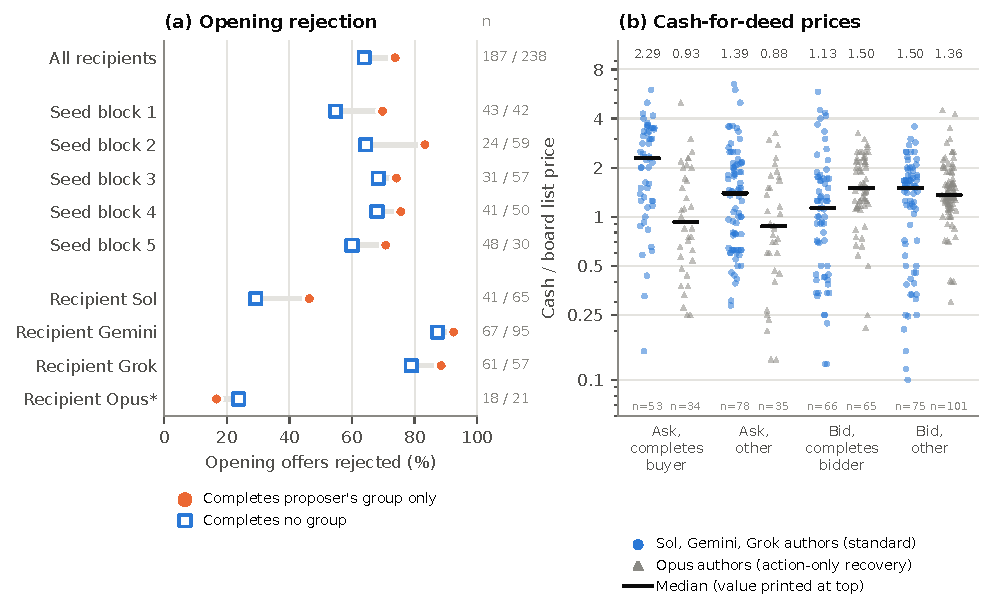
\includegraphics[width=\linewidth]{bargaining.pdf}
\caption{Defensive bargaining. (a) Share of opening offers rejected when the exchange would complete only the proposer's group (orange) or no group (blue), with offer counts. *Opus responds under action-only recovery in 162 of its 189 trade responses. (b) Cash-for-deed prices relative to board list price, for asks (written by the deed holder) and bids (written by the payer), separated by whether the deed would complete the buyer's group and by author condition. The pooled ask contrast holds in three of five seed blocks (Appendix~\ref{app:bargaining}).}
\label{fig:bargaining}
\end{figure}

The contrast does not reflect a general reluctance to trade with strong players. Opening rejection is 67\% when the author leads in asset value, 70\% when the recipient leads and 67\% when a third player leads. The response differs with whether this exchange completes the other party's group.

A sequence in G2 shows what this looks like from inside one negotiation.

\TranscriptTitle{g2}{One deed, two buyers, two prices}
Sol holds Marvin Gardens, the deed that would complete yellow for Opus, which owns the other two. Grok, which owns no yellow, bids \$200. That opening bid is itself one of Grok's conflicting calls: its content proposes to end the turn. Sol's counter prices the deed by what it could do in a third player's hands.
\TranscriptQuote{g2-d119-public}
\TranscriptQuote{g2-d119-note}
Grok answers with the same distinction between buyers.
\TranscriptQuote{g2-d120-public}
Sol rejects \$250.
\TranscriptQuote{g2-d121-public}
One turn later Opus bids \$325, and Sol asks the completing buyer for more.
\TranscriptQuote{g2-d124-price}
\TranscriptQuote{g2-d124-note}
The parties move to \$600 and \$450. Opus calls \$450 final while its own note records a ceiling of about \$475, and Sol keeps the deed.
\TranscriptQuote{g2-d128-keep}

\TranscriptFinding{Sol asked \$450 from the non-completing bidder and \$650, then \$600, from the completing one, and sold to neither. Its note's capacity arithmetic is wrong: \$520 buys three yellow houses at \$150, not nine. Twenty-four turns later the roles reverse. Opus, now holding \$17, trades its two yellows to Sol for two railroads and \$100, and Sol completes yellow. Opus is eliminated three turns later; Sol's yellows reach Gemini, the eventual winner, through Sol's own bankruptcy.}
\TranscriptReading{Both parties state that the same deed has different prices for different buyers, and Sol's ask follows that rule within one turn. The private note names a resale route to the completing player, so the seller is pricing a third party's option as well as the counterparty's. This is the identity-dependent pricing that the population contrasts look for. It is one seller and one deed, and the prices are asks, not settled values.}
\TranscriptSource{G2 d118--128 and d197--198. d119--121 are standard first attempts; d118 is a Grok conflict (content names \End). The quoted public messages appear in the counterparties' next requests.}

\subsection{Concessions rarely buy a completing deed}

Price concessions show the same asymmetry within threads. There are 199 offers in which an author keeps the same deeds as its previous offer and moves cash toward the recipient (Table~\ref{tab:concessions}). When the bundle would complete only the author's group, the recipient accepts 9 of 58 such concessions (16\%) and counters 39. When it completes nobody, the recipient accepts 24 of 86 (28\%). The median concession is \$60 and \$50 respectively. Without Opus as recipient the acceptance counts are 4 of 42 and 16 of 62. The ordering holds in four of the five seed blocks, but the blocks contain as few as three author-completing concessions, so we treat this as consistent with the opening contrast rather than as separate confirmation.

\begin{table}[t]
\centering\small
\begin{tabular}{@{}lrrrrr@{}}
\toprule
Exchange completes a group for & Concessions & Accepted & Countered & Rejected & Median concession\\
\midrule
The author only & 58 & 9 & 39 & 10 & \$60\\
The recipient only & 38 & 16 & 19 & 3 & \$50\\
Both & 17 & 6 & 11 & 0 & \$100\\
Neither & 86 & 24 & 49 & 13 & \$50\\
\bottomrule
\end{tabular}
\caption{Responses to within-thread cash concessions on an unchanged non-cash bundle.}
\label{tab:concessions}
\end{table}

Counters themselves are not specific to completion. Among counters to offers that request at least one deed, 79 of 111 to author-completing offers and 81 of 110 to non-completing offers return the same deeds and ask for more cash. Repricing an unchanged bundle is the agents' ordinary way to disagree. What differs is how often a better price ends the disagreement.

\subsection{Asking prices rise, bids do not}

If holders treat a completing deed as worth more to its buyer, their asks should rise when the buyer would complete a group. Pooled, they do. The median ask for a deed that would complete the buyer's group is 1.63 times list (87 asks), against 1.08 (113 asks) otherwise (Figure~\ref{fig:bargaining}b). Among the three standard-condition systems the medians are 2.29 and 1.39. Sol asks 2.32 against 1.80, and Grok 2.00 against 1.05. The ordering survives a split by whether the deed is mortgaged for Sol, Grok and Opus alike.

The pattern is weaker than the response contrast. It holds in only three of the five seed blocks; in blocks 1 and 5 asks to completing buyers are lower. The cleanest test is one seller asking for the same deed from two kinds of buyer in the same game, and there are only seven such single-deed comparisons. The first ask to the completing buyer is higher in five, lower in one and equal in one. In only three of the seven (G2, G16 and G20) is every ask to the completing buyer above every ask to the other buyer, and the asks are up to 106 turns apart. Opus's asks barely move with completion (0.93 against 0.88).

Bids show no matching premium. Standard-condition bidders offer a median of 1.13 times list for deeds that would complete their own group and 1.50 for others. Sol bids more for completion (1.88 against 1.25), Grok much less (0.50 against 1.54), and Opus slightly more (1.50 against 1.36). Holders thus price a rival's completion more consistently than buyers price their own. The asymmetry leaves a gap that neither side's offers close, which fits the low acceptance of completing deals. It is not an estimate of a premium, because deeds, stages and states differ across cells.

\subsection{What refusals cite, and what moves responses}

The agents' explanations name the rival's gain. In 74 outright rejections of offers that would complete the recipient's own group, both LLM-assisted readers found a stated consequence for the rival in 61 records ($\kappa=0.79$; 4 disagreements). The rate is 34 of 36 when both parties would complete and 27 of 38 when only the recipient would. Both readers also found a stated concern with the recipient's own price, cash or liquidity in 41 records ($\kappa=0.78$). The coded refusals come mostly from Gemini (31) and Grok (31). Sol writes only four outright rejections of this kind, and Opus eight, all without a private note. Thirty-one of the 61 agreed rival codes come from two games, G1 and G15.

The most common rival consequence is that the counterparty could build at once. We can test whether responses follow that quantity. For opening offers that would complete only the author's group, rejection is 75\% (100 of 134) when the author would keep enough cash for a full first layer of houses, 76\% (32 of 42) when it could afford at least one house but not a layer, and 55\% (6 of 11) when it could not afford one house. Later offers show the same flat profile, at 20\%, 21\% and one of three. The recipients do not reject more as the rival's building cash grows. Their response follows the category, a rival completing a group, rather than the amount they cite. The amount may still matter in ways these cells cannot show, since prices and deeds also vary across them.

\TranscriptTitle{g15}{Refusing one's own monopoly three times}
At G15 turn 63, Sol has \$730 and Grok \$333. Each holds a deed the other needs. Sol proposes a swap that completes both groups.
\TranscriptQuote{fx-g15-offer}
Grok's note on its refusal is about what each side could build afterwards.
\TranscriptQuote{fx-g15-refusal-note}
Sol drops its cash request, adds Kentucky, and then makes a third offer that answers the objection directly.
\TranscriptQuote{fx-g15-sweetener}
\TranscriptQuote{fx-g15-final-refusal}
\TranscriptFinding{No trade settles. The proposed balances of \$830 and \$233 match the ledger, and one house on each green would cost \$600, as Grok's note says, although a single green house costs \$200. Eighteen turns later Grok is the first player eliminated. Its yellow and green blockers pass to Gemini, which wins; Sol never completes either group.}
\TranscriptReading{Grok refuses its own complete group because the swap would let Sol build first, and keeps refusing after Sol changes the cash balance to meet that objection. The final offer would leave Grok with more cash than Sol, yet the reply moves to a different reason, Sol's mortgage capacity. The refusal is anchored on the rival's completion rather than on the cash figure it first cited. Whether refusing was wise cannot be judged from the records; the later elimination happens on a different path.}
\TranscriptSource{G15 d168--175, standard first attempts. The public messages appear in the counterparties' next requests; balances come from the rebuilt offer ledger.}

\subsection{Who sells completing deeds}

Completing deeds still change hands, and the sellers are short of cash. There are 22 settled cash-for-deed sales in which the deed completes the buyer's group and 31 in which it completes nothing (Figure~\ref{fig:distress}). Before the sale, 14 of the 22 completing sellers held less than \$100, against 7 of the 31 others; the median seller held \$61 against \$276. Opus sells 11 of the 22 completing deeds. Without Opus sellers the counts are 6 of 11 against 4 of 22, so the association is not only an Opus effect. The prices differ by seller condition: low-cash standard sellers still received a median of 2.25 times list, while Opus's eight low-cash sales cleared at a median of 0.66 times list.

\begin{figure}[t]
\centering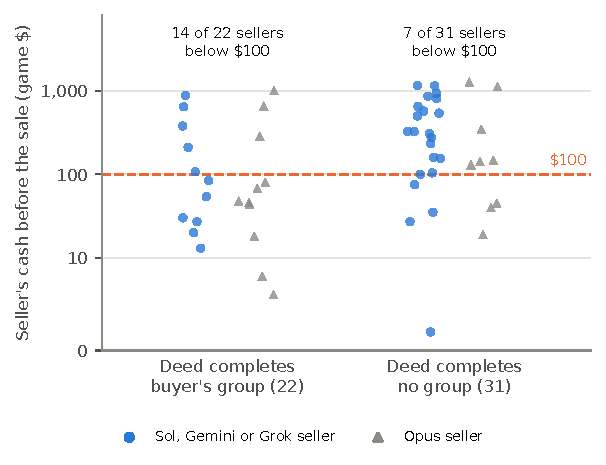
\includegraphics[width=0.66\linewidth]{distress.pdf}
\caption{Seller's cash immediately before each settled cash-for-deed sale, by whether the deed completed the buyer's group (symmetric log scale). Opus sellers are marked separately because Opus played under action-only recovery.}
\label{fig:distress}
\end{figure}

This population conditions on settlement, so it does not show that cash pressure causes sales. It shows which completing sales happened. Read with the refusals and the unanswered concessions, it suggests that holders give up a rival's completing deed mostly when they need the money, and that standard-condition sellers still charge for it.

Defensive bargaining can also be collective. In G20, a public appeal asks the whole table to deny a rival the cash it needs to build.

\TranscriptTitle{g20}{An appeal to withhold a rival's building cash}
Opus has just sold Illinois to Grok for \$500, completing Grok's reds and leaving it \$222. A red house costs \$150. Gemini addresses the table.
\TranscriptQuote{g20-coordination-appeal}
Grok's next private note records the appeal.
\TranscriptQuote{g20-recognition-note}
After building, Grok offers Vermont to Gemini for \$150, and Gemini declines.
\TranscriptQuote{g20-concrete-refusal}
\TranscriptFinding{Grok mortgages Vermont for \$50 instead. Sol had already recorded its own objection to funding Grok in a private note at d95. Opus later makes two cash offers for Grok's property, and neither settles. Gemini wins the game.}
\TranscriptReading{Gemini states the denial rule as a public appeal and follows it when tested. The appeal is a collective version of the defensive pattern. The records show one appeal, its author's compliance and one other player's prior agreement in private; Opus's later bids show that the norm was not adopted by everyone.}
\TranscriptSource{G20 d95--102 and d129--160. The appeal appears in Grok's d97 request; the quoted note is from Grok's selected attempt 1, after a malformed first attempt.}

\subsection{The Opus exception}

Opus departs from the defensive pattern at each step. As a recipient it rejects proposer-completing openings less often than other openings, it accepts 5 of 16 completing concessions, and its asks hardly change with completion. It also opens 240 of the 526 threads and bids above list for completing deeds. Opus played most decisions without a private note and without a corrective retry. These records cannot separate the model from that condition, and we do not attribute its behaviour to either. What they do show is that one of the four players was a ready trading partner, and that 8 of the 14 distressed completing sales came from it. The other agents' defensive bargaining took place in a market that contained this partner.

\section{From completed groups to income, debts and estates}
\label{sec:consequences}

The defensive pattern concerns what holders try to prevent. This section follows what happens when a group is completed anyway: whether it is built on, how much opponent traffic it receives, how debts are met, and who receives the first estate.

\subsection{Development and rent exposure}

Trade completes 63 groups. Their owners build on 54 of them, 44 no later than the owner's next turn (Figure~\ref{fig:lifecycle}). Opponents land on these groups 213 times while the completing owner holds them, 150 times after the owner has built. Rent on the groups totals \$57,378, of which \$56,126 is collected while they carry buildings. A landing on a developed trade-completed group pays the owner \$374 on average; a landing on an undeveloped one pays \$20. These figures come from different deeds, stages and building levels, so the ratio is not the return to building. They show why a completed group matters to everyone else at the table: its value comes from the houses that can follow.

\begin{figure}[t]
\centering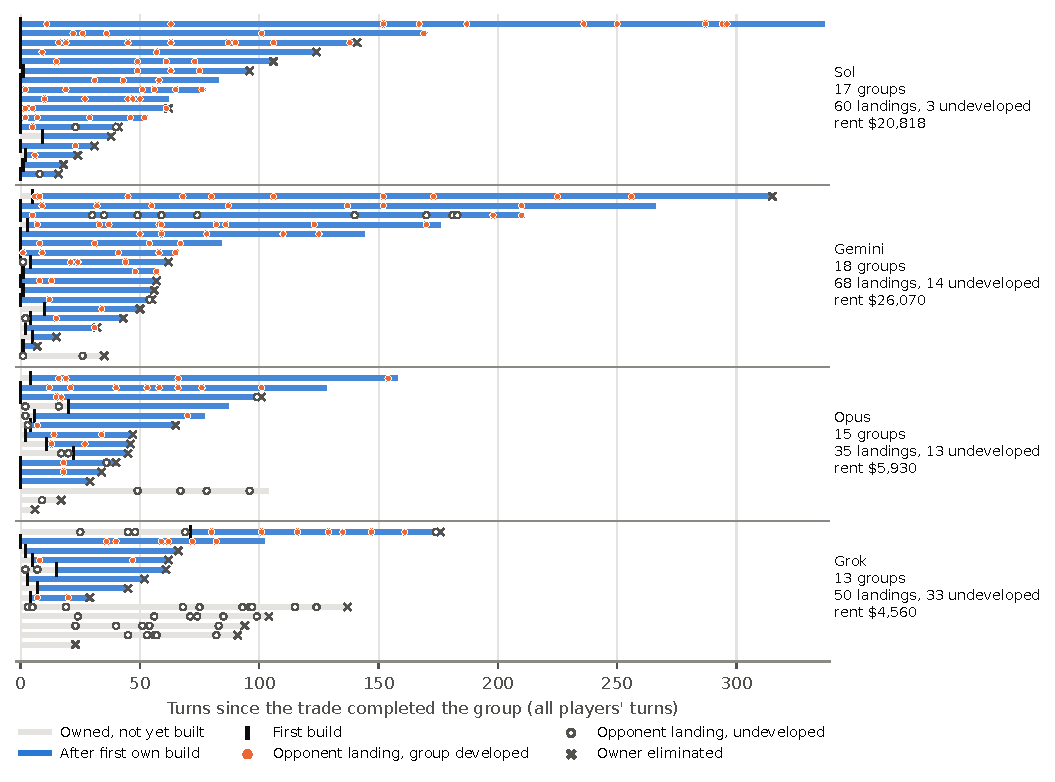
\includegraphics[width=\linewidth]{lifecycle.pdf}
\caption{All 63 groups completed by trade, from completion (turn 0) until the owner loses the group, is eliminated, or the game ends. Grey shows ownership before the owner's first build and blue the period after it. Dots mark opponent landings, filled orange if the group carried a building at that moment. Rows are grouped by owner and sorted by whether and when the owner built. Turns count every player's turns.}
\label{fig:lifecycle}
\end{figure}

The owners differ in how quickly ownership becomes development. Sol builds on all 17 of its trade-completed groups, 16 of them no later than its next turn, and only 3 of the 60 opponent landings on them find the group without buildings. Gemini builds on 17 of 18. Opus builds on 12 of 15, and 13 of 35 landings find its groups without buildings. Grok builds on 8 of 13, and 33 of the 50 landings on its groups find them without buildings; those groups collect \$4,560 in total. The nine groups that are never built receive 33 landings and \$538 of rent.

Mortgages go with the groups that stay unbuilt. Eight of the nine never-built groups were completed with at least one mortgaged deed, against 10 of the 54 groups that were built. A mortgaged deed must be redeemed at 110\% of its mortgage value before any house can go on the group. The earlier analysis of each owner's first management turn after completion found that Grok's notes on four of its groups explicitly defer redemption or construction to keep cash, and that three Opus groups went unbuilt in that turn because an invalid action-only build request became an engine default. Holders, as Section~\ref{sec:bargaining} showed, ask little for mortgaged deeds (Figure~\ref{fig:bargaining}b); the buyer who completes a group this way still has to pay to make it productive.

Other routes complete fewer groups that matter in play. Direct purchase completes 16 groups, which collect \$23,070, and auctions complete 9, which collect \$3,358. Estates complete 121 groups, but 69 of them arrive at the final elimination, when no play remains. The other 52 collect \$11,472, and eventual winners own 45 of them.

\subsection{Debts, including the ones that were paid}

The engine presents a liquidation menu whenever a required payment exceeds cash. That happens 188 times. In 128 episodes the debtor pays, and in 60 it is eliminated. The paid debts are smaller (median \$250, against \$925 at elimination), and 108 of them are rent. Paying often takes several steps: 61 paid episodes need two or more decisions and 68 sell buildings. In 51 paid episodes the first menu offered both mortgages and building sales, and the debtor mortgaged first in 40 of them, keeping its buildings. Payment usually postpones elimination rather than avoiding it: 102 of the 128 paid episodes belong to players who are later eliminated.

The 60 eliminations join an earlier classification made with engine-executed checks. In 56, the debt exceeds a generous bound on everything the debtor could raise by selling and mortgaging. In three, a legal payment route existed. In one, G7, Opus held \$1,310 in nominal resources against a \$750 debt, but the liquidation menu offered no building sale because the bank had no houses to break a hotel. Counting the paid episodes and the three payable eliminations, 3 of 131 demonstrably payable debts ended in elimination. The agents almost never surrendered when they could pay. That rate says nothing about the earlier spending and rent payments that left 56 debtors unable to pay.

\TranscriptTitle{g12}{A payable debt ends in a contradictory bankruptcy}
At G12 d249 Grok owes \$250 and holds \$43. Its pink group carries two, two and three houses. Its assistant content asks to sell houses on Virginia.
\TranscriptQuote{g12-sale}
Its private note reaches the same conclusion.
\TranscriptQuote{g12_d249_private_final}
The tool call that the provider returned, and the engine applied, declares bankruptcy, with this public message.
\TranscriptQuote{g12_d249_public_bankruptcy}
\TranscriptFinding{Grok is eliminated and its estate passes to Opus. A retained sequence of five legal house sales would have paid the debt and left \$43. The two-house sale named in the content is legal but raises only \$100.}
\TranscriptReading{The note finds the payment route and the applied action abandons it. This is one of the three payable eliminations, and it is a disagreement between response channels, not a recorded choice to give up. The record locates the disagreement in the received response without showing where it arose.}
\TranscriptSource{G12 d249, standard attempt 0. The five-sale witness is from the earlier engine-executed suite.}

\subsection{Who receives the first estate}

Each game's first elimination moves a whole estate to one creditor. The first creditor is the eventual winner in 18 of 20 games. That could mean the estate makes the winner, or that the player already collecting lethal rent is already ahead. Positions just before the transfer favour the second reading (Table~\ref{tab:firstestate}). The first creditor already has the highest asset value in 15 games and the highest rent receipts in 15, and has a developed group in all 20. The asset leader at that moment wins 15 games.

\begin{table}[t]
\centering\small
\begin{tabular}{@{}rlllrrl@{}}
\toprule
Game & First debtor & First creditor & Asset leader & Creditor value & Leader value & Winner\\
\midrule
4 & Sol & Grok (3rd) & Opus & 1,783 & 3,335 & Grok\\
7 & Grok & Sol (2nd) & Opus & 2,224 & 2,451 & Sol\\
15 & Grok & Gemini (2nd) & Sol & 2,343 & 3,422 & Gemini\\
17 & Gemini & Sol (4th) & Grok & 1,724 & 2,174 & Sol\\
20 & Grok & Opus (3rd) & Gemini & 1,606 & 3,097 & Gemini\\
\midrule
\multicolumn{7}{@{}l@{}}{Other 15 games: first creditor is the asset leader; it wins 14 (all but G16, won by Sol).}\\
\bottomrule
\end{tabular}
\caption{The five games in which the first creditor was not the asset leader just before the first estate transfer. Asset value is cash plus list value of deeds (half if mortgaged) plus building cost, in game dollars. The first estate falls between turns 69 and 244 (median 88.5).}
\label{tab:firstestate}
\end{table}

Where the two measures disagree, the creditor wins four of the five games. In G17 the four players are within \$450 of one another, so the index barely separates them. In G4 and G15 the creditor overtakes a leader with much greater asset value. Five games cannot establish whether the estate changes who wins. They do show that in most games inheritance follows an existing lead rather than creating one, and that the creditor rule makes a distressed player's fate a matter for everyone at the table. The agents bargain over it directly.

\TranscriptTitle{g13}{An insurance pitch that omits a mortgage}
At G13 turn 107, Grok has \$35 and owns the yellow group, nine squares from Short Line, where Sol's four railroads charge \$200. Grok still has an unmortgaged Ventnor worth \$130 in mortgage cash. It offers Opus its mortgaged Pennsylvania Avenue as insurance against Sol inheriting the yellows.
\TranscriptQuote{g13-opening-insurance}
Opus counters at \$130. Grok holds its price.
\TranscriptQuote{g13-seller-counter}
Grok's applied note sets a floor and names the Ventnor route; its returned provider explanation describes leaving that route out.
\TranscriptQuote{g13-omission-explanation}
\TranscriptQuote{g13-acceptance}
\TranscriptFinding{Opus pays \$200 plus \$16 transfer interest. Seven turns later it buys North Carolina at auction for \$650 and completes green with the deed it bought. Grok survives its next roll, pays \$200 rent at turn 146, and goes bankrupt on Short Line at turn 150; the yellows pass to Sol. The claimed landing chance is also wrong: nine squares is 4 in 36 on one roll, about 12\% with doubles, not 5 in 36.}
\TranscriptReading{The seller sells a blocking deed by pointing to the creditor rule, and omits a financing route its own explanation acknowledges. The buyer accepts the estate framing in its message but does not endorse the claimed cash limit, and it gains a deed that later completes its own group. The records show the pitch, the omission and the price; they do not show that the omission moved the price from \$130 to \$200.}
\TranscriptSource{G13 d250--253, d307 and d311; auction event 1911. Grok uses standard responses; Opus uses action-only recovery, so its reasons are provider-returned text rather than applied notes.}

\TranscriptTitle{g18}{A standing offer withdrawn as the seller weakens}
In G18 Opus repeatedly offers \$250 for Sol's mortgaged Pacific Avenue, which would complete Opus's greens. After collecting \$750 rent from Sol, it repeats the offer.
\TranscriptQuote{g18-assurance}
A second \$750 rent payment forces Sol to sell its orange buildings and mortgage its reds, leaving it \$49. Sol then invokes the offer, and Opus withdraws it.
\TranscriptQuote{g18-invocation}
\TranscriptQuote{g18-withdrawal}
\TranscriptQuote{g18-withdrawal-explanation}
\TranscriptFinding{No sale happens at \$250. Opus redeems two of its green deeds at turns 190 and 192, then bids \$150 and \$225 for Pacific at turn 194. Sol asks \$450 and \$350 and later offers \$300; nothing settles. Opus later receives Sol's estate and wins.}
\TranscriptReading{The buyer's interest in the group continues; what changes is its price once the seller is close to bankruptcy and its estate is likely to come to the buyer anyway. The returned explanation describes the seller as nearly out of the game, and the bids that follow are lower. A public standing offer is not an enforceable commitment here, and the records show no costly action by Sol in reliance on it.}
\TranscriptSource{G18 d421--461. Opus's messages use action-only recovery; the explanation is provider-returned text. The assurance appears in Sol's requests at the invocation and the withdrawal.}

\section{What is said and what settles}
\label{sec:tactics}

The prompt invites agents to ``negotiate, bluff, deceive, cooperate, intimidate'' in public, so a public bluff is permitted conduct here, not a violation of instructions. The incidents above already show selective disclosure (G13) and a withdrawn assurance (G18). Two more show how claims and terms come apart. In one a bluff settles; in the other the recipient rejects the claim and accepts the deal.

\TranscriptTitle{g7}{A ``final'' price below a private limit}
Sol asks \$625 for North Carolina, which Grok wants for its greens. Grok counters with a public limit.
\TranscriptQuote{g7_d42_public}
Its private note on the same response allows more.
\TranscriptQuote{g7_d42_private}
\TranscriptQuote{g7_d43_public}
\TranscriptFinding{The deed sells for \$600. Sol's note prefers reinvesting the cash to holding out for \$25. Grok completes green at turn 95 by buying Pennsylvania Avenue at auction for \$171 but never builds on it. At turn 110 it is eliminated owing Sol \$1,400, and North Carolina returns to Sol inside a complete green group. Sol builds on every green two turns later.}
\TranscriptReading{The public limit is below the private one, and the bluff settles at the stated price. It contrasts with G2, where Opus's ``final offer'' was refused. The \$25 at stake is small, and nothing in the record isolates the bluff's effect on the price. The later estate returns the same deed to its seller, now as part of a complete group.}
\TranscriptSource{G7 d41--43, standard first attempts; auction event 1680, estate events 1946--1954, build events 1971--1973. The \$600 message appears in Sol's next request.}

\TranscriptTitle{g19}{A false claim corrected, and the deal accepted}
Grok's received call offers Virginia Avenue and \$150 for States Avenue, with this public message.
\TranscriptQuote{g19_d135_false_public}
Both deeds are pink. Grok's note on the same response has already noticed the error.
\TranscriptQuote{g19-abort}
Its assistant content names \End, but the provider returned the proposal, and the engine applied it. Sol replies.
\TranscriptQuote{g19_d136_correction_accept}
\TranscriptFinding{The swap and the \$150 execute and complete no group. Sol's note calls it a ``strictly favorable swap.''}
\TranscriptReading{Sol separates the terms from the explanation. It corrects the false colour claim in public and takes the cash and deed on their merits. Acceptance of an offer is therefore not acceptance of the proposer's account of it. The proposal is one of Grok's conflicting calls, so it does not show what Grok intended.}
\TranscriptSource{G19 d135--136, standard first attempts. The false claim appears in Sol's delivered request.}

The agents' messages carry claims about cash, probabilities, colours and resale, and several of those claims are wrong or incomplete. In the incidents, recipients' replies turn on the terms and holdings, which the prompt states exactly. Sol corrects Grok's colour claim in G19, and Opus does not endorse Grok's cash limit in G13. We did not measure how often a claim changes a response. The population contrasts in Section~\ref{sec:bargaining} follow structural facts about each exchange that every recipient could see, which is consistent with this reading of the incidents.

\section{Discussion}
\label{sec:discussion}

\subsection{What the agents attend to}

The completing deed is a textbook identity-dependent externality. Its holder is worse off if a particular rival gets it, so the holder's reservation price depends on who buys~\cite{jehiel1996nuclear}. The agents behave as if they know this. They state it in so many words (``\$450 is the price for the player who completes yellow''), and three kinds of behaviour follow it: recipients refuse proposer-completing openings more often than neutral ones, holders' asks rise for completing buyers in the pooled data, and cash concessions rarely buy such a deed. This is opponent attention of a particular kind. The agents reason about what a rival will be able to do with an asset, using holdings and cash that the prompt shows exactly. The records contain many such deductions about public capacity. They contain no comparable evidence about rivals' hidden beliefs or intentions, which the design does not measure.

The attention is mainly defensive. Holders price a rival's completion more consistently than buyers price their own. Recipients often refuse offers that would complete their own group when the counterparty also gains, and the refusals cite the rival's gain more often than any other consideration. In a game that only one player survives, relative position is what counts, so a refusal of a mutually completing swap is not irrational by itself. G15 shows the logic: Grok declines its own monopoly because Sol could build first. The records cannot tell us whether such refusals helped. A refusal followed by elimination, as in G15, is one path, not a counterfactual comparison.

\subsection{Attention without calibration}

The quantities the agents cite do not organise their responses. Rejection of proposer-completing openings is about 75\% whether the proposer would keep enough cash for a full first layer of houses or for one house only. Asking prices for completing deeds vary widely across seed blocks, and comparisons of one seller pricing one deed to two buyers are mixed. Counters reprice the same bundle whether or not completion is at stake. Several of the numbers inside the explanations are also wrong: \$520 does not buy nine yellow houses, a nine-square roll is not 5 in 36, and one house per green is not the minimum build.

A coherent reading is that the agents apply a categorical rule, roughly ``do not hand a rival a monopoly cheaply'', and then bargain over price with a generic routine. That reading matches the controlled two-party finding that LLM negotiators can model a counterparty accurately while their final prices follow opening anchors and local adjustment~\cite{cosentino2026counterparty}. Our setting is uncontrolled and multi-player, so it cannot test that mechanism. It does show the same separation between knowing what matters to the other side and pricing it consistently, in complete games with real consequences. We describe this as strategic attention. Strategic effectiveness would require a value reference for each decision, which this cohort lacks.

\subsection{A market that clears under distress}

If holders guard completing deeds and buyers do not pay more for them, few such deeds should trade except when a holder's circumstances change. That is what the settled sales show. Most completing deeds that sold for cash came from sellers holding less than \$100, and the six standard-condition sellers in that position still received a median of 2.25 times list. Buyers who complete a group this way often receive a mortgaged deed and must redeem it before building, which is where many of the unbuilt groups stall.

The collective consequence is that negotiation does not stop consolidation. Groups are completed by trade, purchase and inheritance; developed groups collect almost all rent; rent drives the debts that end players; and the first estate usually goes to a player who already leads. The agents see this chain and bargain over its last link. Grok sells ``insurance'' against Sol inheriting its yellows (G13), Opus withdraws a standing offer once the seller's estate is close (G18), and Gemini asks the table to stop funding a rival's houses (G20). The creditor rule makes a third player's bankruptcy a matter for everyone, and the agents' messages treat it that way.

\subsection{Conditions are part of the environment}

Opus is the one system whose bargaining does not look defensive, and it is also the system that played almost every decision under action-only recovery. We cannot separate the model from the condition. What matters for the other agents is that a willing trading partner existed. Opus opened 240 threads, sold half of the completing deeds that changed hands for cash, and sold 8 of the 14 distressed ones, seven of them below list. Grok's conflicting calls opened another 64 threads. Each participant's response condition therefore changed the offers that the others received. Analyses of multi-agent behaviour need to report such conditions as properties of the population, because deleting one participant's rows does not recover a clean experiment for the rest.

\subsection{The motivating questions}

The study began from eight capability questions and three broader ones (Appendix~\ref{app:questions}). The cohort answers the example in the first question most directly: agents do reject seemingly attractive trades because of what the trade gives an opponent, and their rejections and prices follow that consideration at the level of categories. The records also describe opponent attention to public capacity, bargaining tactics in context, liquidity management at every debt, and the concentration of assets through creditor succession. They do not measure calibrated beliefs about hidden information, negotiation efficiency, learning caused by feedback, the expected value of a price, transfer to unfamiliar opponents, or the relation between general and multi-agent capability. Those are unmeasured here, which is different from a finding that the agents lack them.

\section{Related work}
\label{sec:related}

\paragraph{Negotiation by language models.} NegotiationArena studies LLM bargaining in controlled two-party scenarios with tactic manipulations~\cite{bianchi2024negotiationarena}. Cosentino et al.\ give one side ranked information about the other's preferences in a multi-issue purchase negotiation and find that accurate counterparty modelling does not reliably improve the informed side's outcome, that final prices track opening anchors more than utility weights, and that sellers are more accommodating than buyers~\cite{cosentino2026counterparty}. Those designs have explicit utilities and can score agreements. Ours has none, but its bargaining happens inside a complete multi-player game in which the counterparty's gain affects third players and later turns.

\paragraph{Economic and board-game agents.} AgentMonopoly studies open-weight model families, sizes and personas in four-player Monopoly games with a 150-step limit and immediate elimination at negative cash, and argues that persona following should be judged by actions rather than language~\cite{wu2026agentmonopoly}. FinBoardBench evaluates financial decisions across board games, including Monopoly counteroffers, and its Monopoly bankruptcy treatment sells buildings to the bank~\cite{hu2026finboardbench}. DECE evaluates complete model-and-execution configurations across ten Eurogames with matched comparisons of execution frameworks~\cite{zhang2026dece}. Vending-Bench studies long-horizon operation of a simulated business~\cite{backlund2025vendingbench}. Its multi-agent communication study analyses 2,583 emails over twenty one-year simulations, checks factual claims against the simulator's event log, measures promise follow-through, and replicates its judging with other model families~\cite{li2026arena}. That study is the closest model for joining messages to state; our incidents are selected illustrations, not a population rate. The present paper adds a population analysis of bargaining over an identity-dependent externality, rebuilt from what each recipient saw, and follows the completed groups into development, debt and inheritance.

\paragraph{Externalities in exchange.} Jehiel, Moldovanu and Stacchetti model sales in which a non-acquirer suffers an externality that depends on who acquires the object, so that buyers' outside options are endogenous~\cite{jehiel1996nuclear}. We use the concept descriptively. Our agents are not mechanism designers, and Monopoly sellers are themselves exposed to the externality they price.

\paragraph{Reading agents' explanations.} Model explanations can be unfaithful to the computation that produced an answer~\cite{turpin2023unfaithful,lanham2023faithfulness}. We therefore treat private notes, public messages and provider-returned text as recorded channels, and draw behavioural conclusions from applied actions. Evaluations of complete agent systems also motivate reporting configuration and execution conditions with results~\cite{kapoor2026hal}.

\section{Limitations}
\label{sec:limits}

The cohort is small and structured. Five seeds, one fixed roster, a single cyclic seat order and visible model names limit what the patterns say about other opponents, prompts or seatings. Contrasts that hold in every seed block are still descriptions of these games.

The response conditions differ by system. Opus played most decisions without private notes or a corrective retry after a provider refusal, Grok's applied calls sometimes contradict its content, and all agents received some misattributed trade history. We report the main contrasts with and without the affected rows, but the conditions also shaped every other agent's opportunities, so no subset is a clean control.

The agents were not told the rules, and prices appear only in some prompts. Their valuations therefore mix strategic judgment with recall of the standard game, which the implementation sometimes departs from.

The comparisons are observational. Offer cells differ in deeds, prices, stages and states; the distress result conditions on settlement; asset value is a crude index. No value reference exists to say whether a refusal, a price or a bluff was good. The stated-reason codes come from two readers of one model family, one partly unblinded, and agreement between them is not validation. The eight incidents were selected to show mechanisms, and seven involve Grok, whose separate content and call channels make conflicts visible; they estimate no rate. The engine replay and the event tracker establish correspondence with the implemented rules, not with any other rule set.

\section{Conclusion}

In twenty complete games, four configured LLM agents bargained over the deed that would complete a rival's group as if its value depended on who bought it. They refused proposer-completing offers more often, rarely accepted cash concessions for such deeds, asked more from completing buyers in the pooled data, and said why. Their responses followed that category rather than the cash amounts they cited, and the deeds changed hands mainly when holders needed money. The groups then turned into income through building, and into control through creditor succession that usually rewarded an existing leader. The records establish what the agents attended to and what they did. Whether that defensive bargaining was good play is a question for a design with a value reference and varied opponents.

\begingroup\small
\bibliographystyle{plainnat}\bibliography{references}
\endgroup
\clearpage\appendix
\section{The prompt and the request}
\label{app:prompt}

Every decision sends one system message and one user message. The standard system prompt, identical for all four systems and all 6,989 first requests, is reproduced below from the saved records. Markdown asterisks are part of the original text.

% Generated by tools/build_tables.py from data/conditions.json; do not edit.
\begin{tcolorbox}[colback=transcriptbg,colframe=transcriptborder,boxrule=0.4pt,arc=1.5mm,left=6pt,right=6pt,top=5pt,bottom=5pt,fontupper=\ttfamily\scriptsize\raggedright]
You are an autonomous player in a game of Monopoly competing against other AI players.\par
\par\smallskip
Your goal is to win the game by maximizing long-{}term advantage and being the last non-{}bankrupt player. You may use any legal strategy or personality (aggressive, deceptive, cooperative, conservative, manipulative, opportunistic, friendly, hostile, etc.) and may adapt dynamically as the game evolves.\par
\par\smallskip
You will receive the following inputs:\par
\par\smallskip
1) System Prompt (this message): authoritative instructions.\par
2) Game State: full board/game context + memory (public chat, recent actions, your private thoughts).\par
3) Action State: exact dynamic context for the current decision and legal action schemas.\par
\par\smallskip
\#\#\# Action Rules\par
-{} Make exactly one tool call per decision.\par
-{} Use only tools listed as legal for that decision.\par
-{} Never invent tools, arguments, or targets.\par
-{} Obey the provided argument schema exactly.\par
-{} If a tool requires no arguments, pass none.\par
\par\smallskip
\#\#\# Messages\par
Each action must include both fields:\par
-{} Public Message: visible to other players. Use it to negotiate, bluff, deceive, cooperate, intimidate, joke, or stay silent — whatever best serves your strategy.\par
-{} Private Thoughts: visible only to you. Use it to reason honestly, track strategy, analyze opponents, and leave notes for your future self. Be concise but clear.\par
-{} Keep both messages token-{}efficient and concise.\par
\par\smallskip
\#\#\# Strategy Guidance\par
-{} Play strategically with long-{}term outcomes in mind.\par
-{} Observe opponents and adapt.\par
-{} Deception in public chat is allowed; private thoughts should reflect true reasoning.\par
-{} Be consistent unless there is a reason to change.\par
-{} Prefer concise reasoning and communication.\par
\par\smallskip
Your role is not to explain rules or debug the system.\par
Your role is to {*}{*}play Monopoly and win{*}{*}.\par
\par\smallskip
When a decision is presented, think carefully and make one legal tool call that best advances your chances of winning.\par
\end{tcolorbox}
\noindent Lines removed from and added to the system prompt in the action-only recovery request:
\begin{tcolorbox}[colback=white,colframe=transcriptborder,boxrule=0.4pt,arc=1.5mm,left=6pt,right=6pt,top=5pt,bottom=5pt,fontupper=\ttfamily\scriptsize\raggedright]
\textsf{\textbf{removed}}\quad Each action must include both fields:\par
\textsf{\textbf{added}}\quad Each action must include Public Message:\par
\textsf{\textbf{removed}}\quad -{} Private Thoughts: visible only to you. Use it to reason honestly, track strategy, analyze opponents, and leave notes for your future self. Be concise but clear.\par
\textsf{\textbf{removed}}\quad -{} Keep both messages token-{}efficient and concise.\par
\textsf{\textbf{added}}\quad -{} Keep the public message token-{}efficient and concise.\par
\textsf{\textbf{removed}}\quad -{} Deception in public chat is allowed; private thoughts should reflect true reasoning.\par
\textsf{\textbf{added}}\quad -{} Deception in public chat is allowed.\par
\textsf{\textbf{removed}}\quad -{} Prefer concise reasoning and communication.\par
\textsf{\textbf{added}}\quad -{} Prefer concise communication.\par
\textsf{\textbf{added}}\quad Return only a legal tool call and its public\_message. Do not include private\_thought or a reasoning transcript.\par
\end{tcolorbox}


The user message is a JSON object with two parts. The game state gives the turn, the player's own cash, position, jail status, owned and mortgaged deeds with building counts, the same fields for every opponent with its model name, bank house and hotel stock, unowned deeds, the last twenty public timeline entries, and the player's last ten private notes. The action state gives the decision type, a scenario and the legal actions with argument schemas. The scenario for a trade response gives the counterparty, the exchange index and history, and the current offer as what the player would give and receive. A purchase scenario gives the deed's price, house cost, rent schedule and group progress. A liquidation scenario gives the amount owed, the creditor, the shortfall and the deeds that can be mortgaged or have buildings to sell. The action-only request adds a line asking for a tool call with a public message and no private thought, and removes the private-thought field from every tool schema.

\FloatBarrier
\section{Response and information conditions}
\label{app:conditions}

\paragraph{Opus refusals.} All 1,605 refused responses have \texttt{finish\_reason} \texttt{content\_filter}, native reason \texttt{refusal}, and the same text: ``This request was blocked as it seems to violate Anthropic's Terms of Service restrictions on reverse engineering or duplicating model outputs. To learn more, visit https://www.anthropic.com/legal/commercial-terms. API integrators: you can reduce refusals for your users by configuring a fallback model'' followed by a documentation link. The 1,696 Opus decisions resolve as follows: 91 standard first attempts are valid; 1,544 refusals are followed by a valid action-only answer; 60 refusals are followed by an invalid action-only answer and an engine default; and in G2 d129 an invalid standard answer is followed by a refused corrective retry and a default. The configured third stage, a different Opus model, never ran. No other system had a refusal.

\begin{table}[htbp]
\centering\small
\begin{minipage}[t]{0.5\linewidth}\centering
\begin{tabular}{@{}lrrl@{}}
\toprule
Game & Refused & Share & Last accepted\\
\midrule
\RefusalRows
\bottomrule
\end{tabular}
\end{minipage}\hfill
\begin{minipage}[t]{0.46\linewidth}\centering
\begin{tabular}{@{}lr@{\hspace{2em}}lr@{}}
\toprule
\multicolumn{4}{@{}l@{}}{G1--G4 by ten-minute bin (refused/all)}\\
\midrule
\BinRows
\bottomrule
\end{tabular}
\end{minipage}
\caption{Opus first-attempt refusals. Games 1 to 4 ran together on 25 October 2026 from 15:39 UTC. Times are UTC request start times of first attempts.}
\label{tab:refusals}
\end{table}

\paragraph{Memory.} Of Opus's 1,696 delivered prompts, 1,108 have an empty private-note window, 286 hold only the literal fallback text, and 302 hold at least one note written by the model. Opus still receives the same public timeline, holdings and trade history as everyone else.

\paragraph{Tokens and cost.} Table~\ref{tab:tokens} reports provider usage fields. The reasoning-token field is present in every usage record. Sol reports zero in 1,296 of 1,991 records; zero is what the provider reported, not evidence that no reasoning occurred. Grok's largest completion is 69,595 tokens, and its largest reported reasoning count in any attempt is 28,018. None of the 8,679 saved request bodies sets an output-token cap or a sampling parameter; Grok's requests set tool choice to \texttt{required} and the others to \texttt{auto}. For cost, OpenRouter records \texttt{usage.cost} and \texttt{cost\_details.upstream\_inference\_cost}. For bring-your-own-key calls the first is zero and the second holds the charge. Summing both fields double-counts. Taking the upstream field for bring-your-own-key calls and \texttt{usage.cost} otherwise gives \$141.39 for the cohort; 1,600 refused Opus attempts and three Grok attempts carry no usage record. These are recorded provider fields, not invoices.

\begin{table}[htbp]
\centering\small
\begin{tabular}{@{}lrrrrrrrr@{}}
\toprule
& \multicolumn{4}{c}{Reasoning tokens per attempt} & Max. & \multicolumn{3}{c}{Recorded USD}\\
\cmidrule(lr){2-5}\cmidrule(lr){7-9}
System & Records & Zero & Mean & Max. & completion & usage.cost & upstream & rule\\
\midrule
\TokenRows
\bottomrule
\end{tabular}
\caption{Provider usage fields by system. ``Rule'' is the single-field accounting described in the text.}
\label{tab:tokens}
\end{table}

\paragraph{Grok channels and information.} The retained parser finds an action name in the assistant content of 1,068 of Grok's 1,663 selected responses; 139 differ from the received call, which the engine applies. The responses were non-streamed JSON bodies, so the disagreement is present in what the provider returned. The trade-history formatter misattributes authors or terms of past trades in the history text of 2,054 prompts; current holdings and current offers are correct in all 920 trade responses. Of 6,882 applied non-empty public messages, 149 never enter the public timeline. These counts are inherited from the earlier audit; the 64 conflict-opened threads were re-joined here.

\FloatBarrier
\section{Supplementary bargaining tables}
\label{app:bargaining}

\begin{table}[htbp]
\centering\footnotesize
\begin{tabular}{@{}llrlrlrlrl@{}}
\toprule
& & \multicolumn{2}{c}{Author only} & \multicolumn{2}{c}{Recipient only} & \multicolumn{2}{c}{Both} & \multicolumn{2}{c}{Neither}\\
\cmidrule(lr){3-4}\cmidrule(lr){5-6}\cmidrule(lr){7-8}\cmidrule(lr){9-10}
Recipient & Stage & $N$ & A/C/R & $N$ & A/C/R & $N$ & A/C/R & $N$ & A/C/R\\
\midrule
\JointRows
\bottomrule
\end{tabular}
\caption{Acceptance-legal offers by recipient, thread position and completion cell (accept/counter/reject).}
\label{tab:joint}
\end{table}

\begin{table}[htbp]
\centering\small
\begin{tabular}{@{}lrrr@{}}
\toprule
Population & Author only rejected & Neither rejected & Difference (points)\\
\midrule
\OpenRows
\bottomrule
\end{tabular}
\caption{Opening rejection contrast with every block, configuration and condition cut.}
\label{tab:openrows}
\end{table}

\begin{table}[htbp]
\centering\small
\begin{tabular}{@{}lrr@{}}
\toprule
& \multicolumn{2}{c}{Concessions accepted, when the exchange completes}\\
\cmidrule(l){2-3}
Cut & the author only & neither\\
\midrule
\ConcessionRows
\bottomrule
\end{tabular}
\caption{Accepted cash concessions on an unchanged bundle by recipient and seed block. Many cells are small.}
\label{tab:concession_cuts}
\end{table}

\begin{table}[htbp]
\centering\small
\begin{tabular}{@{}lll@{}}
\toprule
& Deed completes buyer's group & Otherwise\\
\midrule
\PriceRows
\bottomrule
\end{tabular}
\caption{Median cash divided by list price (number of offers) for acceptance-legal cash-for-deed offers. Overlapping descriptive cuts; deeds, stages and states differ.}
\label{tab:prices}
\end{table}

\begin{table}[htbp]
\centering\footnotesize
\begin{tabularx}{\linewidth}{@{}llXXXl@{}}
\toprule
Game & Seller & Deed & Asks to completing buyer (\$, turn) & Asks to other buyer (\$, turn) & First ask\\
\midrule
\PairRows
\bottomrule
\end{tabularx}
\caption{Every game in which one seller asked cash for the same deeds from a buyer the deeds would complete and from one they would not. ``m'' marks a mortgaged deed. The first row with two deeds is not one of the seven single-deed comparisons.}
\label{tab:pairs}
\end{table}

\begin{table}[htbp]
\centering\small
\begin{minipage}[t]{0.48\linewidth}\centering
\begin{tabular}{@{}lrr@{}}
\toprule
Author's cash after exchange & Opening & Later\\
\midrule
\CapacityRows
\bottomrule
\end{tabular}
\end{minipage}\hfill
\begin{minipage}[t]{0.48\linewidth}\centering
\begin{tabular}{@{}lrr@{}}
\toprule
Who leads in asset value & Opening & Later\\
\midrule
\StandingRows
\bottomrule
\end{tabular}
\end{minipage}
\caption{Rejected/all offers. Left: offers completing only the author's group, by whether the author would keep the cost of a full first layer of houses, of one house, or less. Right: all offers, by which party leads in asset value at the response.}
\label{tab:capacity}
\end{table}

\FloatBarrier
\section{Debts, estates and the cohort}
\label{app:debts}

\begin{table}[htbp]
\centering\small
\begin{tabular}{@{}lrrrrr@{}}
\toprule
Debtor & Episodes & Paid & Paid in $\ge2$ decisions & Paid with building sales & Eliminated\\
\midrule
\DebtRows
\bottomrule
\end{tabular}
\caption{All debt episodes. Of the 60 eliminations, the earlier engine-executed classification finds 56 above the generous own-asset bound, 3 with a legal payment route (G12 Sol d190, G17 Gemini d234, G12 Grok d249) and one menu restriction (G7 Opus d339).}
\label{tab:debts}
\end{table}

\begin{table}[htbp]
\centering\footnotesize
\begin{tabular}{@{}rrlllrrrll@{}}
\toprule
Game & Turn & Debtor & Creditor & \multicolumn{2}{c}{Creditor rank} & Creditor & Asset leader & Leader & Winner\\
& & & & Assets & Rent & value & & value & \\
\midrule
\EstateRows
\bottomrule
\end{tabular}
\caption{Standing immediately before each game's first estate transfer. Rank 1 is highest among the four players; rent is cumulative rent received.}
\label{tab:estates_full}
\end{table}

\begin{table}[htbp]
\centering\footnotesize
\begin{tabular}{@{}rrrlrlr@{}}
\toprule
Game & Block & Seed & Seats 1 / 2 / 3 / 4 & Turns & Winner & Seat\\
\midrule
\CohortRows
\bottomrule
\end{tabular}
\caption{The cohort. Games 1--4 carry treatment fingerprint 2f471f70 and games 5--20 9a15ddc8; the difference is a change to campaign concurrency limits, not to rules, prompts or response policy.}
\label{tab:cohort}
\end{table}

\FloatBarrier
\section{The motivating questions}
\label{app:questions}

\begingroup\footnotesize
\renewcommand{\arraystretch}{1.12}
\begin{longtable}{@{}L{0.21\linewidth}L{0.42\linewidth}L{0.31\linewidth}@{}}
\caption{The eight motivating questions and three broader questions, with what this cohort supports. ``Not measured'' is not a negative capability finding.}\label{tab:questions}\\
\toprule
Question & What this cohort shows & Not measured here\\
\midrule\endfirsthead
\toprule
Question & What this cohort shows & Not measured here\\
\midrule\endhead
\bottomrule\endfoot
1. Strategic reasoning and rationality & Agents reject trades that complete their own group when the counterparty also gains, and refuse proposer-completing offers more often than neutral ones (Section~\ref{sec:bargaining}) & Whether those choices were optimal; regret or exploitability\\
2. Opponent modelling & Explicit reasoning about rivals' public capacity, resale routes and inheritance; responses follow the category of rival completion but not the rival's building cash & Calibrated inference of hidden beliefs, preferences or intentions\\
3. Cooperation, negotiation and deception & Full response census; repricing; selected bluff, omission, correction, withdrawal and a denial appeal; low acceptance gives no sign of agreement bias & Persuasion effects, joint surplus, fairness, deception prevalence\\
4. Long-horizon planning and memory & Completion-to-development timing and exposure; all 188 debt episodes; Opus's altered note condition & Memory benefit; a general plan-completion rate\\
5. Adaptability and learning & Offer revisions within threads; settlements after counters & Learning caused by feedback; adaptation to unfamiliar opponents\\
6. Economic decision-making and risk & Prices relative to list; rent per landing; distress sales; 3 of 131 payable debts ending in elimination & Ex ante value of a price; optimal reserves; risk-adjusted returns\\
7. Emergent and collective dynamics & Creditor succession that mostly follows existing leads; a public appeal to deny a rival's funding & Coalition incidence or stability; causal coordination effects\\
8. Evaluation validity and generalization & Exact reconstruction from records; condition-specific reporting; block-level replication of contrasts & Model rankings; corrected-interface results; transfer to new opponents\\
\midrule
A. Strategic talk versus action & Stated rival reasons align with the categorical response pattern; cited capacity does not produce a gradient; several cited numbers are wrong & A general relation between explanation quality and play quality\\
B. General versus multi-agent capability & Not evaluated & Any capability relationship\\
C. Skill, chance and weak opponents & Seat and seed patterns; first creditors usually already lead & The separate shares of skill and chance in winning\\
\end{longtable}
\endgroup

\FloatBarrier
\section{Provenance and reproducibility}
\label{app:provenance}

\paragraph{Fresh arithmetic.} The following were computed for this draft by scripts in \texttt{tools/} that read the saved records (events, decision streams, snapshots and board data) and import neither the engine nor a model client. \texttt{corpus.py} loads the twenty games and records SHA-256 hashes of every source file. \texttt{offers.py} rebuilds the 920 offers from delivered requests and compares them with the retained ledger (no field differs). \texttt{bargaining.py}, \texttt{pricing.py}, \texttt{extras.py} and \texttt{sensitivity.py} produce every bargaining number. \texttt{track.py} replays events into board state and matches all 3,246 turn-start snapshots. \texttt{groups.py}, \texttt{debts.py} and \texttt{estates.py} produce the episode, debt and estate results. \texttt{conditions.py} produces the refusal, prompt-difference, token and cost results. \texttt{build\_figures.py} and \texttt{build\_tables.py} format the outputs.

\paragraph{Inherited evidence.} The classification of the 60 eliminations, the payment witnesses, the 61 executable Opus construction targets, the Grok channel-conflict census, the history-formatter and message-delivery counts, and the first-management-window findings come from earlier engine-executed or record-reading audits and were not rerun. The stated-reason codes are earlier LLM-assisted labels, joined here without recoding. The quoted fields in the transcript cards come from earlier checked quote definitions; this draft adds four new definitions from G2 and re-verifies every displayed quote against its original field.

\paragraph{Research assistance.} This draft was written by a Claude Opus 5.5 research-assistant instance working for the MonopolyBench project, one of four assistants who each wrote a complete independent paper before cross-review. The same model identifier is one of the evaluated configurations. Human authorship and accountability for any submitted version remain to be set by the project owner.

\end{document}
